 % The main file for CAMP reports
 % Don't put any content in here. 
 % Don't even include content files by using \input or \inlcude. 
 % Put your content to TEXT.TEX or include it there using \input.
 % Uses:
 %		SETTINGS.TEX	contains the settings for this document
 %		COMMANDS.TEX	contains commands which can be used while writing
 %		INFO.TEX			contains the author, title and so on for the cover
 %		COVER.TEX			formats the front cover of the document
 %		ABSTRACT.TEX	contains the abstract to be included (if needed)
 %		TEXT.TEX			contains the actual content of the document
 %		BIB.BIB				containt the BibTeX entries for the document
 
 
%% Draft document mode
%% Final document
\documentclass[11pt,a4paper,bibtotoc,idxtotoc,headsepline,footsepline,footexclude,BCOR12mm,DIV13]{scrbook}

%\documentclass[11pt,a4paper,bibtotoc,idxtotoc,headsepline,footsepline,footexclude,BCOR20mm,DIV10]{scrbook}

% KOMA-Optionen:
%  bibtotoc: include bibliography in table of contents
%  idxtotoc: include index in table of contents
%  headsepline: use horizontalline under heading
%  BCOR: binding correcion (Bindungskorrektur) (e.g.: BCOR5mm)
%  DIV: Number of sheet sections (used for layout) (e.g.: DIV12) 



% include title and author information for the cover
% Set here the title, authors and other stuff to be used for the cover
% This file is used by MAIN.TEX

% set title, authors and stuff for the cover
\def\doctype{Diplomarbeit in Informatik}
\def\title{Applications of Deep Learning in Natural Language Processing in \\
German for Document Classification and Information Extraction }
\def\titleGer{Die grosse Arbeit}
\def\author{Miguel Fernando Cabrera Granados}
\def\date{March 15, 2014}

% text to appear in the footer
\def\footertext{}


% include settings
% Included by MAIN.TEX
% Defines the settings for the CAMP report document

\renewcommand{\sectfont}{\normalfont \bfseries}        % Schriftart der Kopfzeile

% manipulate footer
\usepackage{scrpage2}
\pagestyle{scrheadings}
\ifoot[\footertext]{\footertext} % \footertext set in INFO.TEX
%\setkomafont{pagehead}{\normalfont\rmfamily}
\setkomafont{pagenumber}{\normalfont\rmfamily}

%% allow sophisticated control structures
\usepackage{ifthen}

% use Palatino as default font
\usepackage{palatino}

% enable special PostScript fonts
\usepackage{pifont}

% make thumbnails
\usepackage{thumbpdf}

%to use the subfigures
\usepackage{subfigure}


\usepackage{colortbl}

\usepackage{acronym}


%% show program code\ldots
%\usepackage{verbatim}
%\usepackage{program}

%% enable TUM symbols on title page
\usepackage{styles/tumlogo}


\usepackage{multirow}

%% use colors
\usepackage{color}

%% make fancy math
\usepackage{amsmath}
\usepackage{amsfonts}
\usepackage{amssymb}
\usepackage{textcomp}
\usepackage{yhmath} % f�r die adots 
%% mark text as preliminary
%\usepackage[draft,german,scrtime]{prelim2e}

%% create an index
\usepackage{makeidx}

% for the program environment
\usepackage{float}

%% load german babel package for german abstract
%\usepackage[german,american]{babel}
\usepackage[german,english]{babel}
\selectlanguage{english}
\sloppy

% use german characters as well
\usepackage[latin1]{inputenc}       % allow Latin1 characters

% use initals dropped caps - doesn't work with PDF
\usepackage{dropping}


\usepackage{styles/shortoverview}
%----------------------------------------------------
%      Graphics and Hyperlinks
%----------------------------------------------------

%% check for pdfTeX
\ifx\pdftexversion\undefined
 %% use PostScript graphics
 \usepackage[dvips]{graphicx}
 \DeclareGraphicsExtensions{.eps,.epsi}
 \graphicspath{{figures/}{figures/review}} 
 %% allow rotations
 \usepackage{rotating}
 %% mark pages as draft copies
 %\usepackage[english,all,light]{draftcopy}
 %% use hypertex version of hyperref
 %\usepackage[hypertex,hyperindex=false,colorlinks=true,hidelinks]{hyperref}
\else %% reduce output size \pdfcompresslevel=9
 %% declare pdfinfo
 %\pdfinfo { 
 %  /Title (my title) 
 %  /Creator (pdfLaTeX) 
 %  /Author (my name) 
 %  /Subject (my subject	) 
 %  /Keywords (my keywords)
 %}
 %% use pdf or jpg graphics
 \usepackage[pdftex]{graphicx}
 \DeclareGraphicsExtensions{.jpg,.JPG,.png,.pdf,.eps}
 \graphicspath{{figures/}} 
 
 %% Load float package, for enabling floating extensions
 \usepackage{float}
 
 %% allow rotations
 \usepackage{rotating}
 %% use pdftex version of hyperref
 \usepackage[pdftex,colorlinks=true,linkcolor=black,hidelinks,citecolor=red,%
 anchorcolor=red,urlcolor=red,bookmarks=true,%
 bookmarksopen=true,bookmarksopenlevel=0,plainpages=false%
 bookmarksnumbered=true,hyperindex=false,pdfstartview=%
 ]{hyperref}

\usepackage{longtable}
%
%\usepackage[pdftex,colorlinks=false,linkcolor=red,citecolor=red,%
% anchorcolor=red,urlcolor=red,bookmarks=true,%
% bookmarksopen=true,bookmarksopenlevel=0,plainpages=false%
% bookmarksnumbered=true,hyperindex=false,pdfstartview=%
% ]{hyperref}
\fi




%% Fancy chapters
%\usepackage[Lenny]{fncychap}
%\usepackage[Glenn]{fncychap}
%\usepackage[Bjarne]{fncychap}

%\usepackage[avantgarde]{quotchap}

% set the bibliography style
%\bibliographystyle{styles/bauermaNum}
%\bibliographystyle{alpha}
\bibliographystyle{plain}


% include commands
% Commands to be used within the TUM report document
% Included by MAIN.TEX
% Please include your own cool commands here. 
% Be only sure to comment it sufficiently so others can use it.

%-------------------------------------------------------------
%                      Own Commands
%-------------------------------------------------------------


%-------------------------------------------------------------
% math stuff -------------------------------------------------

% nice R, N, C
\newcommand{\nat}{\mathbb{N}}
\newcommand{\real}{\mathbb{R}}
\newcommand{\compl}{\mathbb{C}}



% norm
\newcommand{\norm}[1]{\left\| #1 \right\|}

% un demi
\newcommand{\half}{\frac{1}{2}}

% parantheses
\newcommand{\parenth}[1]{ \left( #1 \right) }
\newcommand{\bracket}[1]{ \left[ #1 \right] }
\newcommand{\accolade}[1]{ \left\{ #1 \right\} }
%\newcommand{\angle}[1]{ \left\langle  #1 \right\rangle }

% partial derivative: %#1 function, #2 which variable
% simple / single line version
\newcommand{\pardevS}[2]{ \delta_{#1} f(#2) }
% fraction version
\newcommand{\pardevF}[2]{ \frac{\partial #1}{\partial #2} }

% render vectors: 3 and 4 dimensional
\newcommand{\veciii}[3]{\left[ \begin{array}[h]{c} #1 \\ #2 \\ #3	\end{array} \right]}
\newcommand{\veciv}[4]{\left[ \begin{array}[h]{c} #1 \\ #2 \\ #3 \\ #4	\end{array} \right]}

% render matrices: 3  dimensional (arguments in row first order)
\newcommand{\matiii}[9]{\left[ \begin{array}[h]{ccc} #1 & #2 & #3 \\ #4 & #5 & #6 \\ #7 & #8 & #9	\end{array} \right]}
%DOESN'T WORK,DON'T KNOW WHY \newcommand{\mativ}[16]{\left[ \begin{array}[h]{cccc} #1 & #2 & #3 & #4 \\ #5 & #6 & #7 & #8 \\ #9 & #10 & #11 & #12 \\ #13 & #14 & #15 & #16 \end{array} \right]}


%-------------------------------------------------------------
%-------------------------------------------------------------


%-------------------------------------------------------------
% some abreviations ------------------------------------------
\newcommand{\Reg}{$^{\textregistered}$}
\newcommand{\reg}{$^{\textregistered}$ }
\newcommand{\Tm}{\texttrademark}
\newcommand{\tm}{\texttrademark~}
\newcommand {\bsl} {$\backslash$}

%-------------------------------------------------------------
%-------------------------------------------------------------


%-------------------------------------------------------------
% formating --------------------------------------------------

% Theorem & Co environments and counters
\newtheorem{theorem}{Theorem}[chapter]
\newtheorem{lemma}[theorem]{Lemma}
\newtheorem{corollary}[theorem]{Corollary}
\newtheorem{remark}[theorem]{Remark}
\newtheorem{definition}[theorem]{Definition}
\newtheorem{equat}[theorem]{Equation}
\newtheorem{example}[theorem]{Example}
\newtheorem{algorithm}[theorem]{Algorithm}

% inserting figures
\newcommand{\insertfigure}[4]{ % Filename, Caption, Label, Width percent of textwidth
	\begin{figure}[htbp]
		\begin{center}
			\includegraphics[width=#4\textwidth]{#1}
		\end{center}
		\vspace{-0.4cm}
		\caption{#2}
		\label{#3}
	\end{figure}
}




% referecing figures

\newcommand{\refFigure}[1]{ %label
	figure \ref{#1}
}
\newcommand{\refChapter}[1]{ %label
	chapter \ref{#1}
}

\newcommand{\refSection}[1]{ %label
	section \ref{#1}
}

\newcommand{\refParagraph}[1]{ %label
	paragraph \ref{#1}
}

\newcommand{\refEquation}[1]{ %label
	equation \ref{#1}
}

\newcommand{\refTable}[1]{ %label
	table \ref{#1}
}




\newcommand{\rigidTransform}[2]
{
	${}^{#2}\!\mathbf{H}_{#1}$
}

%code, in typewriter
\newcommand{\code}[1]
 {\texttt{#1}}

% comment that appears on the border - very practical !!!
\newcommand{\comment}[1]{\marginpar{\raggedright \noindent \footnotesize {\sl #1} }}

% page clearing
\newcommand{\clearemptydoublepage}{%
  \ifthenelse{\boolean{@twoside}}{\newpage{\pagestyle{empty}\cleardoublepage}}%
  {\clearpage}}


%-------------------------------------------------------------
%-------------------------------------------------------------


\newcommand{\etAl}{\emph{et al.}\mbox{ }}




%\makeindex
	%% inter line spacing
%\linespread{1.0}

\makeglossary




\begin{document}

	\frontmatter
	
	
	% The front cover for the TUM report document.
% Included by MAIN.TEX


%--------------------------------------------------
% The Front Cover
%--------------------------------------------------

% The front cover for the TUM document.
% Included by MAIN.TEX


%--------------------------------------------------
% The Front Cover
%--------------------------------------------------

% correct BCOR - undo at the end !!!
\def\bcorcor{0.15cm}
\addtolength{\hoffset}{\bcorcor}

\thispagestyle{empty}

 \vspace{4cm}
\begin{center}
	       \oTUM{4cm}
	   
	   \vspace{5mm}     
	   \huge FAKULT{\"A}T F{\"U}R INFORMATIK\\ 
	   \vspace{0.5cm}
	 \large DER TECHNISCHEN UNIVERSIT{\"A}T M{\"U}NCHEN\\
    \vspace{1mm}
        
	\end{center}
		

\vspace{15mm}
\begin{center}

   {\Large \doctype}

  \vspace{20mm}
  
  {\huge\bf \title}\\%[3ex]
  
  
  \vspace{15mm}
  
  
  {\LARGE  \author}
  
  \vspace{10mm}
  
  \begin{figure}[h!]
  \centering
   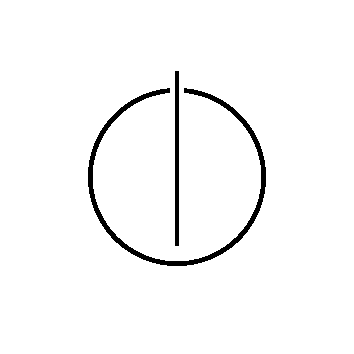
\includegraphics[width=4cm]{styles/informat.png}
  \end{figure}
  
  \end{center}
%	\clearemptydoublepage 
%	
%	% The titlepage for the CAMP report document.
% Included by MAIN.TEX


%--------------------------------------------------
% The title page
%--------------------------------------------------

% correct BCOR - undo at the end !!!
\def\bcorcor{0.15cm}
\addtolength{\hoffset}{\bcorcor}

\thispagestyle{empty}

 \vspace{10mm}
\begin{center}
	       \oTUM{4cm}
	   
	   \vspace{5mm}     
	   \huge FAKULT{\"A}T F{\"U}R INFORMATIK\\ 
	   \vspace{0.5cm}
	 \large DER TECHNISCHEN UNIVERSIT{\"A}T M{\"U}NCHEN\\
        
	\end{center}
		

\vspace{10mm}
\begin{center}

   {\Large \doctype}

  \vspace{10mm}
  
  {\LARGE \title}\\
  
  
  \vspace{10mm}
  
  
  {\LARGE  \titleGer}\\
  
  
  \vspace{10mm}

    %\hfill
    \begin{tabular}{ll}
	   \Large Author:     & \Large \author  \\[2mm]
	   \Large Supervisor:    & \Large Prof. Dr. However Wasit \\[2mm]				
	   \Large Advisor:	& \Large Dipl.Inf. Whoever Didit\\[2mm]
	   \Large Date:       & \Large August 15, 2006
	 \end{tabular}
	 
	 \vspace{5mm}
	 
	 \begin{figure}[h!]
  \centering
   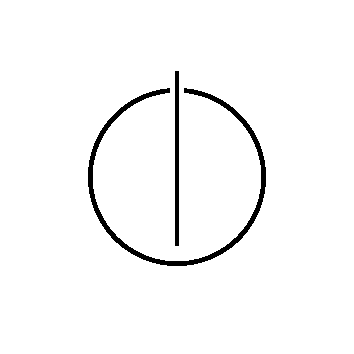
\includegraphics[width=4cm]{styles/informat.png}
  \end{figure}
   

\end{center}

% undo BCOR correction
\addtolength{\hoffset}{\bcorcor}

	
	
%	\input{components/cover_maschmeyer}
	\clearemptydoublepage
	
	% The titlepage for the CAMP report document.
% Included by MAIN.TEX


%--------------------------------------------------
% The title page
%--------------------------------------------------

% correct BCOR - undo at the end !!!
\def\bcorcor{0.15cm}
\addtolength{\hoffset}{\bcorcor}

\thispagestyle{empty}

 \vspace{10mm}
\begin{center}
	       \oTUM{4cm}
	   
	   \vspace{5mm}     
	   \huge FAKULT{\"A}T F{\"U}R INFORMATIK\\ 
	   \vspace{0.5cm}
	 \large DER TECHNISCHEN UNIVERSIT{\"A}T M{\"U}NCHEN\\
        
	\end{center}
		

\vspace{10mm}
\begin{center}

   {\Large \doctype}

  \vspace{10mm}
  
  {\LARGE \title}\\
  
  
  \vspace{10mm}
  
  
  {\LARGE  \titleGer}\\
  
  
  \vspace{10mm}

    %\hfill
    \begin{tabular}{ll}
	   \Large Author:     & \Large \author  \\[2mm]
	   \Large Supervisor:    & \Large Prof. Dr. However Wasit \\[2mm]				
	   \Large Advisor:	& \Large Dipl.Inf. Whoever Didit\\[2mm]
	   \Large Date:       & \Large August 15, 2006
	 \end{tabular}
	 
	 \vspace{5mm}
	 
	 \begin{figure}[h!]
  \centering
   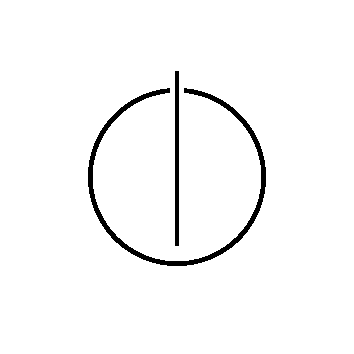
\includegraphics[width=4cm]{styles/informat.png}
  \end{figure}
   

\end{center}

% undo BCOR correction
\addtolength{\hoffset}{\bcorcor}

 
	
	\clearemptydoublepage


\thispagestyle{empty}
\selectlanguage{german}
	\vspace*{0.8\textheight}
	\noindent
	Ich versichere, dass ich diese Diplomarbeit selbst{\"a}ndig verfasst und nur 
	die angegebenen \\Quellen und Hilfsmittel verwendet habe.
	
	\vspace{15mm}
	\noindent
	M{\"u}nchen, den \today \hspace{5cm} \author
\selectlanguage{english}
\newpage
	
	\clearemptydoublepage
\phantomsection
\addcontentsline{toc}{chapter}{Acknowledgements}	


%\chapter*{Acknowledgements}

\vspace*{2cm}

\begin{center}
{\Large \bf Acknowledgments}
\end{center}

\vspace{1cm}




If someone contributed to the thesis... might be good to thank them here.
	
	% Abstract for the TUM report document
% Included by MAIN.TEX


\clearemptydoublepage
\phantomsection
\addcontentsline{toc}{chapter}{Abstract}	





\vspace*{2cm}
\begin{center}
{\Large \bf Abstract}
\end{center}
\vspace{1cm}

The success of machine learning algorithms  depends on the 
representation of the data used.  Specific domain knowledge can be used to
design good representations. However, these representations are limited to a
specific problem  or task, and to the amount of available labeled data.
Another approach is to automatically learn  generic priors that can be used in different
tasks and context. In the field of natural language processing, recent work
has been done in obtaining such priors by learning useful vector representation of
words from unlabeled data. The representations can then be used to improve
existing natural language processing systems.  These word vectors are  obtained using special neural network architectures   
 trained on billions of tokens. However, most of these models  are learned
and evaluated on English language corpora.       In this work,
\textit{Word2vec}, a recent neural network based  toolkit for learning word
representations is used on German language data. The goal is to evaluate the
learned representations of words in different language processing and information
retrieval tasks. In particular, a semantic-syntactic  evaluation set  is
constructed for the German language. In addition to that, the
learned word vector representations are used as features for a classifier of German
language business documents. The learned features outperformed existing handcrafted features and
performed  similar to other state-of-the-art approaches.




%%% Local Variables: 
%%% mode: latex
%%% TeX-master: "../main.tex"
%%% End:


        % Abstract for the TUM report document
% Included by MAIN.TEX


\clearemptydoublepage
\phantomsection
%\addcontentsline{toc}{chapter}{Abstract}	



\vspace*{2cm}
\begin{center}
{\Large \bf Zusammenfassung}
\end{center}
\vspace{1cm}

Auf Deutsch oida!

	\tableofcontents
  
        %\clearemptydoublepage

\phantomsection
\addcontentsline{toc}{chapter}{Outline of the Thesis}

\begin{center}
	\huge{Outline of the Thesis}
\end{center}




%--------------------------------------------------------------------
\section*{Part I: Introduction and Theory}

\noindent {\scshape Chapter 1: Introduction}  \vspace{1mm}

\noindent  This chapter presents an overview of the thesis and it purpose. Furthermore, it will discuss the sense of life in a very general approach.  \\

\noindent {\scshape Chapter 2: Theory}  \vspace{1mm}

\noindent  No thesis without theory.   \\

%--------------------------------------------------------------------
\section*{Part II: The Real Work}

\noindent {\scshape Chapter 3: Overview}  \vspace{1mm}

\noindent  This chapter presents the requirements for the process.

	\mainmatter
	
	
		% ---------------------------------------------------------------------------
		%
		%Introduction and Background Theory
		%
		% ---------------------------------------------------------------------------
		\part[Introduction and Theory]{Introduction and Theory}
		\label{part:introAndBackgroundTheory}

                \chapter{Introduction}
\label{chapter:Introduction}


From the early days of computers, people have dreamed about machines with intelligence. Computers able to exhibit complex behavior and able to solve tasks assigned by users. If we assume that this problem is too difficult to solve immediately, we can think of several step that will lead towards the development of intelligent machines. One of the first tasks to solve is the one of language understanding, i.e. giving the machine to process and understand human language. This by definition is a hard task even for human beings, as natural language is inherently ambiguous.


Current computational language modeling techniques are based on statistical
measurements and hardcoded rules. Although they perform fairly well in
several tasks, they are far from achieving human like results in many natural
language processing problems. One way to try to achieve human like behavior
in a machine is to emulate the way of human brain works. This is the main
idea behind the initial use of neural networks in the early days of
artificial intelligence in the 60s and 70s. The last decade has seen a
revival of this trend via  \textit{Deep Learning} approaches. \textit{Deep Learning} tries to learn useful high-level representations of data using raw data via hierarchical architectures. This is similar in principle to the theories of brain development proposed by the cognitive neuroscientists in the early 1990s.

In the field of natural language processing, most of the research  has
focused on  trying to obtain words representation that allow to extract
meaning from unlabeled text, mostly in English language.  However,  English
lack of the morphological complexity exhibited by other Germanic and
non-Germanic languages such as German and Spanish. Therefore, it  is of
interest to evaluate what information can extract these models from
morphological richer languages. Besides that, one the performance of these
representation of words is assesed, it is important to design or adapt
machine learning system that can take advantage of these representations.


 % Even if these models have achieved to generate representation containing  interesting relationships among words, there are not still a clear way to use them for improving many existing tasks.


%There are t

% 
%The goal of this thesis is to describe new techniques that have been developed to overcome the simple n-gram models that still %remain basically state-of-the-art today. To prove usefulness of the new approaches, empirical results on several standard data %sets will be extensively described. Finally, approaches and techniques that can possibly lead to automatic language learning %by computers will be discussed, together with a simple plan how this could be achieved.


% current language modeling techniques  are based on 
% - Language understanding via language modelling.
% One way to simiulate this behaviour The Turing test was designed by 

% - Alan Turing and the machine (re-write Mikolov thing)
% - Emulating the using neural computation
% - This important because the implications
% - most of the work has been done in english where other languges exists and their differences 
% - Amount of data of data avaitlable on the web
% - Unlabaled thus impoortant to learn from unlabeled data.
% - Text categorization
% - Better language model will lead us to better understanding of human by the machine.


% From the first day of existence of the computers, people were dreaming about artificial intelligence - machines that would produce complex behaviour to reach goals specified by human users. Possibility of existence of such machines has been controversial, and many philosophical questions were raised - whether the intelligence is not unique only to humans, or only to animals etc. Very influential work of Alan Turing did show that any computable problem can be computed by Universal Turing Machine - thus, assuming that the human mind can be described by some algorithm, Turing Machine is powerful enough to represent it.
% Computers today are Turing-complete, ie. can represent any computable algorithm. Thus, the main problem is how to find configuration of the machine so that it would produce desired behaviour that humans consider intelligent. Assuming that the problem is too difficult to be solved immediately, we can think of several ways that would lead us towards intelligent machines - we can start with a simple machine that can recognize basic shapes and images such as written digits, then scale it towards more complex types of images such as human faces and so on, finally reaching machine that can recognize objects in the real world as well as humans can.
% Other possible way can be to simulate parts of the human brain on the level of indi- vidual brain cells, neurons. Computers today are capable of realistically simulating the real world, as can be seen in modern computer games - thus, it seems logical that with accurate simulation of neurons and more computational power, it should be possible to simulate the whole human brain one day.

\section{Motivation and Objectives}

\label{sec:motivation}

The goal of this thesis is to describe deep learning approaches to learn word features,  performing a empirical study of the performance of such representation in the German language and evaluating the applicability of such methods in existing problems, in particular the field of automated text categorization. 

There are two  main motivations behind this objective. First, it is
interesting to evaluate word representation of languages other than English.
This allows measuring  to some degree the generalization power and the ability to extract useful features of these models. Second,  most of the existing data existing is unlabeled. Thus, developing pipelines that allow to take advantage of large amount of available data  is necessary to improve existing systems that  process natural language.  

For that purpose an empirical evaluation of the \textit{Word2vec} model  on German
language corpora has been chosen. \textit{Word2vec} is a tool that by means of
a neural network learns vector representation of words.
\textit{Word2vec} is used  because it has shown to produce representations
that contain rich relationships among words . In the application area, the
field of automatic document classification of German language document has
been selected. The reason for this is two-fold. On one had, the amount  work
has been done in applying such representation  in the general area of
automated document classification is limited. On the other hand, the nature
of the data set chosen,  from which limited amount of document is available;
offer the perfect chance to evaluate the performance obtained by using
features learned from unlabeled data.

%%- natural language and therefore word vector embeddings model has been mostly evalutated using english as the basic language
% - how these perform on toher languages other than english with more complex grammar and sytax is nonethelss important.

% - word2vec has shown to generate interesting word vector maininigting linear relationships. However, up to this date no applications of these word vector model besides some experiments with translation. 
% - This word explores a previous approach to document classificaion using word word vectors but with two particularities. One the exsitince of an already classifier based on handcrafted features, second the language of work is German, that is a highly inflective language. 


\section{Structure of the Thesis}
\label{sec:structure-thesis}

The theoretical foundation required for the understanding of this thesis is
described in chapter \ref{chap:related_work}. This chapter also gives an
overview about related work in the of language modeling and text
representations.  In particular, it describes the model that led to the
development of \textit{Word2vec}.
 Chapter \ref{chap:word2vec_description} describes in detail the architecture
 \textit{Word2vec}. Afterwards in  chapter \ref{chapter:wor2vec_german}  
 an empirical evaluation of the \textit{Word2vec} model on a German language
 corpus is performed.  Chapter \ref{chap:rel_word2vec_doc_classification} explores the
 application of these representations in the field automated text
 categorization. Finally, in chapter \ref{chap:conclusion_future_work} the
 thesis is concluded and possible future work is outlined.

% 4 guide through the development process of the WAF. Chapter 5 discusses an evaluation of different wifi AP localization techniques. Finally, in chapter 6 the thesis is concluded and an outlook for future work is given.


% \section{Claims of the Thesis}
% \label{sec:claims-of-the-thesis}



 



%%% Local Variables: 
%%% mode: latex
%%% TeX-master: "../main.tex"
%%% End:

                  
\chapter{Related Work}
\label{chap:related_work}

\section{Natural Language Processing}
\label{sec:rel_nlp}

\section{Language Models}
\label{sec:relwork-language-models}

A statistical language model assigns assigns a probability to a sequence of m
words $P(w_1,\ldots,w_m)$ by means of a probability distribution. 
This probability can be obtained from the probability of
each word given the context of words preceding it using the chain rule of probability \cite{Bengio:2008}:

\begin{equation}
\label{eq:lm_probability}
 P(w_1, w_2, \ldots, w_{t-1},w_t) = P(w_1) P(w_2|w_1) P(w_3|w_1,w_2) \ldots 
  P(w_t | w_1, w_2, \ldots w_{t-1}).
\end{equation}

Most probabilistic language models  approximate $P(w_t | w_1, w_2, \ldots
w_{t-1})$ using a fixed context of size $n-1$, i.e. using  $P(w_t | w_{t-n+1}, \ldots w_{t-1})\ ,$.



\section{N-Grams based language models}
\label{sec:n-gram-lm}

\section{Neural Network Language Models}
\label{sec:nnlms-intro}

As its name describes, is a language model based on a \ac{NN}, exploiting their
ability to learn distributed representations to reduce the impact of the
curse of dimensionality \cite{Bengio:2008}. In other words, a \ac{NN} is
used to estimate the probability described  by equation (\ref{eq:lm_probability}) based on a sequence of
previous words.

The advantage  using  distributed representations  is that they allows
the model to generalize well to sequences that are not in the set of training
word sequences, but that are similar in terms of their features. Because neural networks tend to map nearby inputs
to nearby outputs, the predictions corresponding to word sequences with
similar features are mapped to similar predictions. \cite{Bengio:2008,Bengio:2003:NPL:944919.944966}

However, Due to the nature the architecture, many of these models suffer
performance issues the hidden layers and output layer of the \ac{NN} are
generally the bottleneck.  In order to be able to compare the different
models in term of their complexity it is necessary then to define the
complexity of  their architecture. All of these models have a complexity proportional to 
\cite{DBLP:journals/corr/abs-1301-3781}:

\begin{center}
\begin{equation} O = E \times T \times Q,   \end{equation}
\end{center}

where $E$ is number of the training epochs, $T$ is the number of the words in
the training set and $Q$ depends on each architecture. Common choice is $E$ = 3-50 and $T$ up to one billion.
All models are trained using stochastic gradient descent and backpropagation
\cite{Bengio:2003:NPL:944919.944966}\cite{DBLP:journals/corr/abs-1301-3781}.

The following subsection describe each of the most popular  model and their
associated complexity $Q$.

\subsection{Feedforward Neural Network Language Model}
\label{subsec:fwd-neural-net-lm}

% Section \ref{sec:relwork-language-models} described the generalities of
% language models in the context of \ac{NLP}.  In that section we described
% that the 

In the \ac{FNNLM} that was introduced by Bengio
\cite{Bengio:2003:NPL:944919.944966},  the probabilistic prediction $P(w_t | w_{t-n+1}, \ldots w_{t-1})$ described
in equation (\ref{eq:lm_probability}) is obtained as follows. First, each word $w_{t-i}$ (represented
with an integer in $[1,N]$) in the  $n-1$-word context is mapped
to an associated $d$-dimensional feature vector $C_{w_{t-i}}\ ,$ which is
column $w_{t-i}$ of parameter matrix $C\ .$ Vector $C_k$
contains the learned features for word $k\ .$
Let vector $x$ denote the concatenation of these $n-1$
feature vectors:
\begin{equation}
  x = (C_{w_{t-n+1},1}, \ldots, C_{w_{t-n+1},d}, C_{w_{t-n+2},1}, \ldots C_{w_{t-2},d}, C_{w_{t-1},1}, \ldots C_{w_{t-1},d}).
\end{equation}
The probabilistic prediction of the next word, starting from $x$
is then obtained using a standard artificial neural network architecture
for probabilistic classification, using the softmax activation function at the output units (Bishop, 1995):
\begin{equation}
 P(w_t=k | w_{t-n+1}, \ldots w_{t-1}) = \frac{e^{a_k}}{\sum_{l=1}^N e^{a_l}}
\end{equation}
where
\begin{equation}
 a_k = b_k + \sum_{i=1}^h W_{ki} \tanh(c_i + \sum_{j=1}^{(n-1)d} V_{ij} x_j)
\end{equation}
where the vectors $b,c$ and matrices $W,V$ are also
parameters (in addition to matrix $C$). Let us denote
$\theta$ for the concatenation of all the parameters.
The capacity of the model is controlled by the number of hidden units $h$
and by the number of learned word features $d\ .$ 


\begin{figure}[h]
    \centering
    \caption{Feed Forward Neural Network Model Language Model Architecture}
    \label{fig:NNLM_architecture}
\end{figure}

The neural network is trained using a gradient-based optimization algorithm
to maximize the training set \textit{log-likelihood}
\begin{equation}
 L(\theta) = \sum_t \log P(w_t | w_{t-n+1}, \ldots w_{t-1}) .
\end{equation}
The gradient $\frac{\partial L(\theta)}{\partial \theta}$
can be computed using the backpropagation algorithm \cite{Bishop:1995:NNP:525960}, extended
to provide the gradient with respect to $C$ as well as with
respect to the other parameters. 


Note that when calculating  $\frac{\partial L(\theta)}{\partial \theta}$ we have:

\begin{equation}
  \label{eq:nnlm-grad}
  \frac{\partial }{\partial \theta}\text{log}p_{\theta}^{n}(w) =
  \frac{\partial }{\partial \theta} e^{a_k}


\end{equation}
 




\subsubsection{Model Complexity}
\label{sec:sub:sub:bengio_nnlm_complexity}

Figure \ref{fig:NNLM_architecture} is a graphical description of  the model.
It consists of three layers, input, projection and output layers. The N
previous word are encoded using 1-of-$|V|$ encoding, where $|V|$ is the size
of the vocabulary. $N$ previous word representation are concatenated using a
shared projection matrix to the projection layer $P$ (dimensionality $N
\times D$).  This layer is then conected to a hidden layer which is in turn
used to compute the probability distribution over all the words in the
vocabulary resulting in an output layer with dimensionality $|V|$. Therefore,
the computational complexity of each training example is:

\begin{center}
\begin{equation} Q = N \times D + N \times D \times H + H \times V,   \end{equation}
\end{center}

With the dominant term is $H \times V$
\cite{DBLP:journals/corr/abs-1301-3781}. Many solutions are proposed to avoid
the complexity in the last layer. One alternative is to use  hierarchical
versions of the softmax \cite{Morin05hierarchicalprobabilistic,6163930}.
The other alternative is to avoid is to avoid  normalized models by finding
a approximation to find the likelihood gradient \cite{NIPS2013_5165} . If binary tree representations are
used, the number of output units can decrease down to $log_2(V)$. Most
of the complexity will be then caused by  $N \times D \times H$.

% Of input, projection, hidden and output layers. At the input layer, N previous words are encoded
% using 1-of-V coding, where V is size of the vocabulary. The input layer is then projected to a
% projection layer P that has dimensionality N  D, using a shared projection matrix. As only N
% inputs are active at any given time, composition of the projection layer is a relatively cheap operation.


% Note that the gradient on most of $C$
% is zero (and need not be computed or used) for most of the columns of $C\ :$
% only those corresponding to words in the input subsequence have a non-zero gradient.
% Because of the large number of examples (millions to hundreds of millions),
% the only known practical [[optimization algorithm]] for  
% artificial neural networks 
% are online algorithms, such as [[stochastic gradient descent]]: the
% gradient on the log-likelihood of a single example at a time (one word in its
% context) or a mini-batch of examples (e.g., 100 words) is iteratively used to perform
% each update of the parameters.

% In a similar spirit, other variants of the above equations have been proposed (Bengio et al 2001, 2003;Schwenk and Gauvain 2004;Blitzer et al 2005; Morin and Bengio 2005; Bengio and Senecal 2008).

% The different  existing architecture will be described on section BLAH of
% this document.

\subsection{Recurrent Neural Net Language Model}

One of the major issues of the \ac{FNNLM}  approach is that
it has to used a fixed context that need to be specified at training time.
Therefore, the neural network only can see a limited number of preceding words when
predicting the next one.  A language model based on recurrent neural networks  do not use a context
with a size limit.  By using recurrent connection the information cycle
inside the networks for arbitraily long time. the \ac{RNNLM} proposed by
Mikolov use the so-called simple
recurrent neural network model. The network has an input layer $x$, hidden
layer $s$ (also called context layer or state) and output layer $y$. Input to
the network in time $t$ is $x(t)$, output is denoted as $y(t)$, and $s(t)$ is
state of the network (hidden layer). Input vector $x(t)$ is formed by
concatenating vector $w$ representing current word, and output from neurons in
context layer $s$ at time $t - 1$. Input, hidden and output layers are then
computed as follows \cite{conf/interspeech/MikolovKBCK10}:.

\begin{equation} x(t) = (w(t), s(t-1))  \end{equation} 

\begin{equation} s_j(t) = f \left( \sum_{i}{x_i(t)u_{ij}}
  \right)   \end{equation}

\begin{equation} s_j(t) = g \left( \sum_{j}{s_j(t)v_{kj}}
  \right)   \end{equation}


Where   $f(z)$ is \textit{sigmoid} activation function and $g(z)$  is the
traditional   \textit{softmax}. 

Figure \ref{fig:RNNLM_architecture} despicts the architecture of the simple
recurrent neural network this model is based on. Similar to the \ac{FNNLM},    $w(t)$ represents the word in time $t$ encoded using 1-of-$V$ coding.  $s(t-1)$ represents the output values in the
hidden layer from the previous time step. Therefore $x(t)$, the input, has
the size of the vocabulary $V$ and of vector $s(t-1)$. After the network is
trained, the output represent the probability represented by equation (\ref{eq:lm_probability}).  \cite{mikolovphd2012}.

\begin{figure}[hptb!]
    \centering
    \caption{Recurrent Neural Network Language Model Architecture}
    \label{fig:RNNLM_architecture}
\end{figure}

The network is trained by  stochastic gradient descent using the
\textit{backpropagation} algorithm \cite{Bishop:1995:NNP:525960}.


\subsubsection{Model Complexity}
\label{sec:sub:sub:mikolov_rnnlm_complexity}

Assuming that the hidden layer and the word representation share the same
dimensionality with the hidden layer, the complexity per training example of the RNN model is
given by:


\begin{equation} Q = H \times H + H \times V,   \end{equation}

In a similar fashion to the \ac{FNNLM}, the term $H \times V$ can be
efficiently reduced to $H \times log_2(V)$ by using the hierarchical softmax
formulation. Thus, most of the complexity comes $H \times H$.

% Recurrent neural networks do not use limited size of con- text. By using recurrent connections, information can cycle in
% side these networks for arbitrarily long time (see [5]). However, it is also often claimed that learning long-term dependencies by stochastic gradient descent can be quite difficult [6].
% In our work, we have used an architecture that is usually called a simple recurrent neural network or Elman network [7]. This is probably the simplest possible version of recurrent neu- ral network, and very easy to implement and train. The network has an input layer x, hidden layer s (also called context layer or state) and output layer y. Input to the network in time t is x(t), output is denoted as y(t), and s(t) is state of the network (hidden layer). :




% A major deficiency of Bengio’s approach is that a feedfor- ward network has to use fixed length context that needs to be specified ad hoc before training. Usually this means that neural networks see only five to ten preceding words when predicting the next one. It is well known that humans can exploit longer context with great success. Also, cache models provide comple- mentary information to neural network models, so it is natural to think about a model that would encode temporal information implicitly for contexts with arbitrary lengths.


\subsection{Mikolov's Neural Network Language Model}
\label{sec:mikolov-neural-net-model}

Mikolov neural network language model uses additional approach to the one
described back in section \ref{subsec:fwd-neural-net-lm}.  The neural network
architecture is split in two steps. In the first one the architecture trains
a bigram neural network. Given a word $w$ from a vocabulary $V$, the neural
network tries to estimate the the probability distribution of the next word
in the text. Both the input and output are of size $|V|$, were the words a
usually is encoded with 1-of-$K$ encoding, with $K=|V|$.  Theres is one hidden layer of
size $|D|$ has an arbitrary size (reported by the authors  to range from 20-60). As with the
other models, the output layer  is a  softmax layer. The nework is trained
using the standard \textit{backpropagation} algorithm
\cite{conf/icassp/MikolovKBGC09}. 

The second step consiste of  A $N$-gram network. The network is trained in a
similar waym, however the input vector does not encode previous word in
history using 1-of-$K$ encoding, but is formed using $N-1$ projections from
the  bigram network. These projections are the learned weights of dimension
$|D|$ learned by the big-gram network. Figure \ref{fig:mikolov_nnlm_architecture} show a schematic of the
two-network architecture 


\begin{figure}[hptb!]
    \centering
    \caption{Mikolov's Neural Network Language Model Architecture}
    \label{fig:mikolov_nnlm_architecture}
\end{figure}


\subsubsection{Model Complexity}

As this model is formed by two parts, the model complexity depends wheter the
full model is desired to be estimated or not. If one is only interested in
the word representations, i.e. the projections from the big-gram network the
complexity is reduced  by the simplicity of the model, regardless of the
quality of the representation obtained.  As reference the full model
complexity is described: 


\begin{equation} Q_1 = V \times D + D \times V  \end{equation}

\begin{equation} Q_2 =  N \times D \times H + H \times V   \end{equation}

\begin{equation} Q = Q_1 + Q_2
\end{equation}

With $Q_1$ and $Q_2$ the complexity of the bigram network and the $N$-gram
network respectively. Although not mentioned by the authors, efficiency
improvement can be achieved by using hierarchical formulations of the softmax
can be used. If it is used, most of the complexity  lies in the  $N \times D \times
H$ term of $Q_2$.



% \subsection{Mikolov Neural Network Model}



\section{Deep Learning}
\label{sec:deep_learning}


\section{Represenation of Text}
\label{sec:rel_represenation_text}


\subsection{Local Representations}
\label{sec:rel_local_representation}

\subsubsection{N-grams}
\label{sec:sub_ngrams}

\subsubsection{Bag-of-words}
\label{sec:rel_bow}

\subsubsection{1-of-N coding}
\label{sec:1_of_coding}

\subsection{Continuous Representations}
\label{sec:sub_continuous_representation}

\subsubsection{Latent Semantic Analysis}
\label{sec:rel_local_representation}

\subsubsection{Latent Dirichlet Allocation}
\label{sec:rel_lda}

\subsubsection{Distributed Representations}
\label{sec:dis_rep}





%%% Local Variables: 
%%% mode: latex
%%% TeX-master: "../main.tex"
%%% End:
                
\section{Text Categorization}
\label{sec:rel_text_categorization}

The goal of \ac{TC} is to automatically assign, for each
documents, categories selected among a predefined set.
In opposition to the machine learning typical multi-class classification
task which aims at attributing one class among the possible ones to each
example, documents in a text categorization task may belong to several
categories. 
%Sebastiani Ind
% "Sebastiani02"


Formally,  \ac{TC} is the  task of  assigning a bolean value to each pair 
$\left\langle d_{j},c_{j}\right\rangle \in\mathcal{D}\,\, x\,\mathcal{\, C}$
where  $\mathcal{D}$  is a domain of documents and
$\mathcal{C}=\{c_{1},\ldots,c_{|c|}\}$ is a set of predefined categories. A
true value assigned to the pair $\left\langle d_{j},c_{j}\right\rangle $
indicates the decision of filling  $d_{j}$ under the category  $c_{j}$, and
a false value the decision of not filling it under that category \cite{Sebastiani02}. 

More formally the task is to approximate a unknown target function 
 $\breve{\Phi}:\mathcal{D}\,\, x\,\mathcal{\, C}\rightarrow\{T,F\}$  using 
 $\Phi:\mathcal{D}\,\, x\,\mathcal{\, C}\rightarrow\{T,F\}$  such that 
 $\Phi$ and  $\breve{\Phi}$ ``coincide as much as possible'' \cite{Sebastiani02}. 

So far only the binary case has been discussed, however in many realistic
settings there are many possible (mutually exclusive or not) categories in
which a document can be classified. In these stitutation 

 There are two main ways to  tackle
such problem: 1-vs-All and All-vs-All. 

\textbf{TODO: INSERT THE INFORMATION FROM SCIKIT-LEARN PAGES - e.g.
  DESCRIPTION OF 1-vs-All and All vs all}

\ac{TC} relies  heavily on  models that have been developed originally for \ac{IR}.
 the reason of this is that \ac{TC} is a content based document management task,
 and such it shares many characteristics with other IR tasks such as text
 search, specifically \ac{IR}-style document representation  using \ac{BOW} model described in section \ref{sec:rel_bow}.



\subsection{Performance Measures}
\label{sec:sub_performance_measures}

One question that arises after reading the definition of TC is how to measure
 the how well the classifier function  $\breve{\Phi}$ (the approximation or hypothesis) matches the unknown target function  $\Phi$
 (effectiveness).  This is generally measured in terms of the classic IR
 metrics of precision  $P$  and recall  $R$ but adapted to the specific case
 of \ac{TC}. $P$  is defined as the probability that if a given a random document
 $d_{x}$  is classified under the category  $c_{i}$  the classification is
 correct:

 $$P(\breve{\Phi}(d_{x},c_{i})=T\,\,|\,\, P(\Phi(d_{x},c_{i})=T))$$


 Analogously  $R$  is defined as the probability that if a random document 
 $d_{x}$ is ought to be classified under  $c_{i}$,  this decision is taken
 by the classifier function: 

 $$P(\Phi(d_{x},c_{i})=T\,\,|\,\, P(\breve{\Phi}(d_{x},c_{i})=T))$$
 



%%% Local Variables: 
%%% mode: latex
%%% TeX-master: "../main.tex"
%%% End:

		\chapter{Description of the Word2Vec Model }
\label{chap:word2vec_description}


\section{Introduction}
As described in  previous chapter,  continuous language space models have
demonstrated good results across a variety of tasks. Word vector
representation are in some way a byproduct of \ac{NNLM}, as not only the
model itself is learned by the neural network but also the word representation.  As pointed out by
the authors, these continuous word vector representation capture syntactic
and semantic relationship of words not possible to achieve from a discrete
representation of traditional $n$-gram models. Furthermore, these
representation can be used to improve existing \ac{NLP} tasks.

One of the way to learn a \ac{NNLM} is to learn the word vector using a
\ac{NN} with a single hidden layer. Then, these word vectors are used to
train the \ac{NNLM}. In these architecture learns the word vectors without
even constructing the complete language model.  This chapter describes in
detail a recent approach  to efficiently learn
high-dimensional word representation \cite{DBLP:journals/corr/abs-1301-3781}
focusing only in the first part, that is, learning good word representation
representations.

Another interesting architecture of NNLM was presented in [13, 14], where the word vectors are
first learned using neural network with a single hidden layer. The word vectors are then used to train
the NNLM. Thus, the word vectors are learned even without constructing the full NNLM. In this
work, we directly extend this architecture, and focus just on the first step where the word vectors are
learned using a simple model.

\section{Description of The Model}


\section{Optimization Strategies used by Word2vec}
\label{sec:strategies_improve_time}

\subsection{Huffman Coding}
\label{sec:huffman_coding}

Huffman coding is an entropy  encoding algorithm used for lossless data
compression.  It was developed by David A. Huffman while he was a Ph.D.
student at MIT. \cite{huf52}.

Huffan cioding is an algorithm to proce an  optimal symbol code $C$ for a given 
\emph{pmf} $ p = (p_1,....,p_n) $.  Huffman coding builds a tree orderded by frequency.



%%% Local Variables: 
%%% mode: latex
%%% TeX-master: "../main.tex"
%%% End:
                
                

                                
		%
		%% ---------------------------------------------------------------------------
		%%
		%% Fuly Automated Calibration for Ultrasound
		%%
		%%% ---------------------------------------------------------------------------
		\part[Applications]{Applications}
		\label{part:secondP}
                \chapter{Empirical Study of Word Vectors for the German Language}
\label{chapter:wor2vec_german}

%% In this chapter 

%% - What we do in this chapter 

%% - Rationale why we do that how we do it and why

%% - Short descrioption of Experiments

%% Tasks for English and German and comparisson of Gramatical and semantical differences

%% Datasizes and so on

%% - Embedding using t-SNE of German wikipedia (top X)

%% - Embedding using t-SNE of GiniData using top X

%% - Table of the experiments

%% - Analysis of the results 

The previous chapters introduced the concepts and related work  in the fields
of  \ac{NLP}, \ac{NNLM} and vector representation of words. This chapter will
focus on the application of a particular model, namely \textit{Word2Vec}, to
the German language.  

% There art two main reasons that justify the study of the behavior of word
% vector representation in a language as morphologically rich and  inflective
% as German.

Although that  evidence that word vector representation might work
well in other languages other than English has been presented
\cite{DBLP:journals/corr/MikolovLS13}, to the date  there are not in depth studies or empirical evaluations of the
performance of word representation for such languages,  in similar or equivalent tasks as the
ones performed by \cite{DBLP:journals/corr/abs-1301-3781} for the English
language. 

Previous work has shown that  n-gram backoff language models, the state of the art
technique, does not perform  as well for inflectional  languages as they work
for English \cite{conf/icassp/MikolovKBGC09}.  Previous work also shows that
\ac{NNLM} captures  better the complexity of such languages
\cite{conf/icassp/MikolovKBGC09}\cite{DBLP:journals/corr/MikolovLS13},
therefore  is possible that word vectors generated by such model  will 
improve  and simply many \ac{NLP} applications in
these languages as they have been shown to do in
English \cite{collobert:2008} \cite{Turian:2010:WRS:1858681.1858721}.  This makes therefore an initial evaluation of the quality of the word vector
attractive.

The rest of the chapter is divided as follows: The first part described the
selected tasks, the rationale behind the adaption made to fit the German
language and the data set  and the different preprocessing alternatives we
tried. The second part described the training approach as well describe the most
important result of our approach.

%  In this chapter we will
% describe a set of tasks adapted from \cite{DBLP:journals/corr/abs-1301-3781}
% to better match the characteristics of German language. In addition we will
% compare  the performance with English language.


%  As word vectors are generated
% by \ac{NNLM} \cite{Bengio:2003:NPL:944919.944966}, it is expected therefore,
% t

% First  as reported in previous work, n-gram backoff language models, the state of the art
% technique, do not perform  as well for inflectional  languages as they work
% for English \cite{conf/icassp/MikolovKBGC09}. Recent alternatives
% n-gram based models are \ac{NNLM} \cite{Bengio:2003:NPL:944919.944966} described
% in detail in CHAPTER [TODO:REF]. Besides the language model,  \ac{NNLM}
% generate the word  vector representations .

% in this type of languages \cite{conf/icassp/MikolovKBGC09}\cite{DBLP:journals/corr/MikolovLS13}.
% Second, 

% As mentioned before,  vector representations have shown the ability of
% improve existing \ac{NLP} taks 

% -  There is no studying comparing performances in two different languages and
% how the differences between the language and the standard language affects. 



%  [Thurian and
% Other people papers listed on Mikolov]

% - This work have done in english (not studied in depth in high inflectional
% languages) however there are not study which theoritically explains what 

% - There are some evidence of good performance morphologucally rich (highly
% inflective) lanaguage 

% %
%- [On the other hand, n-gram backoff models do not work
% as well for inflectional languages as they work for
% English] \cite{conf/icassp/MikolovKBGC09} 

%  Several alternative model has been proposed based on \ac{NNLM}

% - As the word embeddings are based also en \ac{NNLM} it is expected that
% thereofore works better. 

% - We use in our work German is a morpholgically rich and moderate inflected
% language (CITATION). We want to test evaluate the performance of this
% particular word embeddings. 

% Similar to the English study we define a set of tasks 

% To evaluate a language model is necessary define a set of tasks 
% For that purpose, a equivalent subset of tasks targeted at the German language were
% defined in the same maner as by Mikolov et al.
% \cite{DBLP:journals/corr/abs-1301-3781} do for the English.  


% It is challenging to test and compare different language models base just by
% comparing their algorithm description, furthermore if for the language of
% choosing no standard data set exist. For that purpose a equivalent  to the
% one defined by  has been created. 

% This chapter will describe the experiments performed as well as the data sets
% used to test the model. Additionally, a comparison between

% To test this model for  German,  a equivalent set of semantic and
% syntantic tasks were created in a similar way to the ones defined by Mikolov
% et al \cite{MikolovSCCD13}.

% This chapter describes the experiments and and tasks used to measure  

% IMPORTANT ALSO FOR GINI SET - [Neural networks seem to be very useful for tasks where
% we struggle with inflectional languages and limited data
% amounts. While performance of our implementation is not
% high,  presents various optimization techniques that lead to
% significant improvements in required computational time for
% training and lattice re-scoring.] - \cite{conf/icassp/MikolovKBGC09}

\section{Task Description}


In their original paper \cite{DBLP:journals/corr/abs-1301-3781} the authors
introduced a comprehensive test that contained five types of semantic
questions. In the original data set  there were 8869 semantic and 10675
syntactic questions. To create this set the authors compiled a list of
similar word pairs manually and then they generated the list by
connecting the word pairs. Table~\ref{tab:task_original_en} shows examples 
examples from each category of tasks. 

To evaluate the quality of the word vectors the question  are answer in the
following manner: given the word pairs ($a$, $b$) and ($c$, $d$) a question
is considered to be answered correctly if the for resulting vector $X$ the closest vector measured in
cosine similarity is  $vector(d)$. $X$ is calculated by applying the following
operation $X = vector(b) - vector(a) + vector(c)$.  

 For example  for the words
($``small''$, $''smaller''$ ) and ($''big''$ ,$"bigger"$),
the $vector("bigger")$ should be the closest to the resulting
vector $X$. If the representation of the word in
vector space is good, then it is possible to find the answer using such
operation \cite{DBLP:journals/corr/abs-1301-3781}.

As discussed in the first part of this work, the word representations
capture different types of  similarities among words. Therefore, with the
operation described above,  what is  being
attempted is to answer the question ``\emph{What is the word that is similar to
c in the same sense as b is similar to a?}''. 

% To compare the quality of different versions of word vectors, previous papers typically use a table
% showing example words and their most similar words, and understand them intuitively. Although
% it is easy to show that word France is similar to Italy and perhaps some other countries, it is much
% more challenging when subjecting those vectors in a more complex similarity task, as follows. We
% follow previous observation that there can be many different types of similarities between words, for
% example, word big is similar to bigger in the same sense that small is similar to smaller. Example
% of another type of relationship can be word pairs big - biggest and small - smallest [20]. We further
% denote two pairs of words with the same relationship as a question, as we can ask: ”What is the
% word that is similar to small in the same sense as biggest is similar to big?”

In order to evaluate the performance of the word vectors in the same way but in other language a
similar set of questions  needs to be created. Two approaches might be used
to accomplish this. The words can be translated, either automatically or by hand, or the data set can be
generated from scratch in a similar manner as the original was.  In this work
the translation was performed by hand using a German - English online dictionary \footnote{http://dict.cc} as guide and
verified by two native speakers.

Regardless of the method chosen, some tasks of this set are biased towards
the morphology of English and could not be easily mapped to another language,
and in particular to German. Therefore a simple translation would not be
enough to obtain a equivalent task set for another language. For that reason
each of the original 14 tasks was analyzed to either adapt it to German or
discard it completely. 


\renewcommand{\arraystretch}{1.3}

\begin{table}[h]
  \centering
  \caption{Examples of the original types of syntactic questions in the
    Semantic-Syntactic Word Relationship test as defined 
    by \cite{DBLP:journals/corr/abs-1301-3781}. }
  \label{tab:task_original_en}

  \begin{tabular}{ |l| |c|*{4}{c| |c| c | c }  }

  \hline           
  Type of Relationship &  \multicolumn{2}{c||}{Word Pair 1} &
  \multicolumn{2}{c|}{Word Pair 2} \\  \hline           
  Common capital city & Athens & Greece & Oslo  & Norway \\ 
  All capital cities  & Astana & Kazakhstan &  Harare & Zimbabwe  \\
  Currency & Angola & kwanza & Iran & rial \\  
  City-in-state  & Chicago & Illinois & Stockton & California \\  
  Man-Woman & brother & sister  & grandson & granddaughter \\  \hline  
  Adjective to adverb & apparent & apparently & rapid & rapidly  \\  
  Opposite & possibly & impossibly & ethical & unethical \\  
  Comparative & great & greater & tough & tougher \\  
  Superlative & easy & easiest & lucky & luckiest \\  
  Present participle & think & thinking & read & reading \\  
  Nationality adjective & Switzerland & Swiss & Cambodia  & Cambodian  \\  
  Past tense & walking & walked & swimming & swam \\ 
  Plural nouns  & mouse & mice & dollar & dollars \\  
  Past verbs & work & works & speak  & speaks  \\  \hline  
  
    
  
  
\end{tabular}
\end{table}

\section{Adapting the tasks to the German Language}
\label{sec:adapt_task_german_lang}

Many of  tasks from the original  Semantic Syntactic set of task are language
dependent. In order to adapt them  to the German language  each of different
types of question was evaluated. Some of them can be easily adapted to German
just by translating the respective word. However, some of the them either do
not make sense for German in from the morphology point of view or do not
apply for German. From the original 14 types of questions, the German version only
10 and equivalent set was also constructed for English for performing the
comparison. Below each of the tasks are described in detail along with what
was done to adapt it to German when possible.

\subsection{Common Capital and City and All Capital}
\label{sec:sub_sec_common_capital_country}

This group of question try to solve analogies between country and capitals.
The vector model is asked the semantic relationship \emph{Capital Country}.
For example:  ``\emph{What is the word that is similar to
Germany in the same sense as Paris is similar to France?}''. The model should
answer then the word produce a vector close to ``\emph{Berlin}''. The
difference between the two subsets is that common capital contains
 the 22 most ``\textit{common}'' country - capital word pairs. However the
 criteria for the selection is not defined by the authors of the set. The
 other subset contains country - capital pairs of less known countries such
 as \textit{Ghana  -  Accra} and  \textit{Harare -  Zimbabwe}.

For this task the adaptation was done by simply translating the names from
the English ones to their German counterparts. 

\subsection{Currency}
\label{sec:sub_sec_currency}
For the currency section all of the pairs were translated using the wikipedia
as source for the information. 

\subsection{City in State}
\label{sec:sub_sec_city_in_state}
This group of questions try evaluate the semantic relationship between a city
and a state for cities in the United States of America.  However, the
objective of the experiment is to have a standard,  almost
language independent comparable test set for the word vectors generated by \textit{Word2Vec}, tasks that
are centered in information mostly found in a specific language are not relevant and
will not provide good information about the quality of the vectors. For this
reason the complete tasks group was removed from the dataset. An alternative could have been to replace it with a similar
tasks (e.g. using cities in Germany / Austria). In this case however,  a
comparisson with another language would have been impossible as the
information sources might not contain that information or even the word
themselves.

\subsection{Man-Woman}
\label{sec:sub_sec_man_woman}
This tasks try to evaluate the semantic relationship between words associated
with men and women. For this tasks the equivalent German version of the word
were used for validation a  online German - English dictionary was used.

\subsection{Adjective to Adverb}
\label{sec:sub_sec_adjetive_adverb}
This task models the relationship between an adjective and its correspondent
adverb. However in German this task cannot be applied,  because unlike English,
German does not make a distinction in form between a predicate adjective and
an adverb \cite{durrell2011hammer}. For example in English:

\begin{itemize}
\item The man is quiet. (quiet = adjective)
\item The man sings quietly. (quietly = adverb)
\end{itemize}

Whereas a German speaker would say:

\begin{itemize}
\item Der Mann ist leise. (leise = adjective)
\item Der Mann singt leise. (leise = adverb)
\end{itemize}

For this reason the trained word vector will not be able to differentiate the
roles. Thus, this tasks is removed from the set. 

\subsection{Opposite}
\label{sec:sub_sec_opposite}
This task try to model the \emph{opposite} semantic relationship between words.
Although it may seem relatively easy to adapt this task to German there
things that need to bee taken into account. In German,  not necessarily the
most common ``antonym'' is used nor they have a regulara morphological
structure as in English. For example  in English is usual to form the
opposite by adding the prefix \textit{in} ,  \textit{un} , \textit{im} or
\textit{dis}. In fact, all of the word pairs that appear in the English
version of this set are formed in such way. This is not always true in
German. For example, the opposite for the word  \textit{\"{u}berzeugend} (roughly
translating to \emph{convincing} in English) has not opposite in that form.
The only way to form the opposite is by adding the negation, e.g.
\textit{nicht  \"{u}berzeugend }. Another example would be the pair
\textit{geschmackvoll} - \textit{ geschmacklos}, which are as well opposites,
but where the suffix is the difference.
However, most of the word in these tasks could be also build in a similar
fashion as in the English set, therefore we adapt this task by looking for
the best translations that can be formed with that common structure.

\subsection{Comparative and Superlative}
\label{sec:sub_sec_comparative_sup}

The comparative task  try to model to evaluate the syntactic relationship between a word
and its comparative form, for example the word pairs  \textit{young} and
\textit{younger}. Respectively the superlative task aims to evaluate the
superlative relationship  (e.g. \textit{safe}  and \textit{safest}). 

Many of the words belonging to this data set can be easily translated to
German directly. However, there are some caveats. First, English have many
more words for representing the same semantic concept than German.  English is language from
the family of Germanic languages, therefore shares the common structure
and grammar. However, many words have been borrowed from Latin, expanding the
vocabulary  and in many cases replacing the words from Germanic origin. 
For example, the word \textit{tall}  comes from Old Germanic and  the
word \textit{large} comes from Latin. Both words could be translated to
German as \textit{hoch}. However, the English word  \textit{high} of German
origin can also be translated as \textit{hoch}.
% Another example of this is the German the word  \textit{gross}, that represents
% the quality  of being  \textit{big}, but also \textit{large} or \textit{tall}.
That is a unique concept in German can represent many things in English. 
Give this, only one word is maintained in German and one English representing
the same concept making the number of pairs equivalent.


% To measure quality of the word vectors, we  a comprehensive test set that contains five types
% of semantic questions, and nine types of syntactic questions. Two examples from each category are
%
\subsection{Present Participle}
\label{sec:sub_sec_present_participle}

This tasks try to model the relationship between verbs and its participle
(e.g. \textit{come} -\textit{coming}). In English is used the participle in
much more ways than German: 

\begin{itemize}
\item  To form the progressive (continuous) aspect: Jim was sleeping. as an
  adjective phrase modifying a noun phrase: The man sitting over there is my
  uncle.
\item adverbially, the subject being understood to be the same as that
  of the main clause: Looking at the plans, I gradually came to see where the
  problem lay.
\item  similarly, but with a different subject, placed before the
  participle (the nominative absolute construction): He and I having
  reconciled our differences, the project then proceeded smoothly.
\item more
  generally as a clause or sentence modifier: Broadly speaking, the project
  was successful.

\end{itemize}

In German, unlike English  the present participle is used almost exclusively as an
adjective or adverb and as such are inflected. This is imply that in a model
such as  \textit{Word2Vec} the same word after the declension will be
represented with different words. For the purpose of this tasks, this mean
the is expected to have low number of correct answers.

\subsection{Nationality Adjective and  Plural nouns}
\label{sec:sub_sec_nat_plu}

The nationality adjective tasks model the relationship between a country and
the the adjective representing the nationality. For example, for the word
\textit{Colombia}, the respective adjective is \textit{Colombian}. In German,
the nationality is also an adjective, and as such, it  is inflected based on the
case and genus of the substantive.  For example  \textit{Kolumbianisch} may appear 
inflected as \textit{Kolumbianischer},  \textit{Kolumbianischem},
\textit{Kolumbianische}, etc.  Similar to the participle, many words will
represent the same concept, thus low correct answer rate are expected in this
task.  
The plural nouns task model the relationship of a word and its plural the
proportion of words that are the same plural is higher than English. This is
a factor that will affect the test results because the same word is never taken as a
valid answer. 


\subsection{Past Tense and Plural Verbs}
\label{sec:sub_sec_plural_verbs}
The two task find syntantic relationship between verbs and they past tense
and the conjugation respectively. This relationships does not hold in German,
and therefore are removed from the test.

\section{Summary of Changes} 
Table \ref{tab:summary_of_changes_task} shows a summary of the changes
performed in other to generate a set for the German language.

 \begin{table}[h]
   \centering
   \caption{Summary of changes } 
   \label{tab:summary_of_changes_task}

   \begin{tabular}{ |l|l|  }

   \hline           
   Task  & Action   \\  \hline           
   Common capital city & Translated \\
   All capital cities  & Translated \\
   Currency & Translated  \\ 
   City-in-state   &  Removed - Language dependent \\
   Currency & Translated  \\
   Man-Woman  & Translated  \\
   Adjective to adverb  &  Removed - do not apply in German \\
   Comparative & Translated - Some words removed due to polisemy \\ 
   Superlative & Translated - particle \textit{am} not used \\
   Opposite  & Translated \\
   Present participle & Translated \\
   Plural Nouns  & Translated \\
   Past verbs &  Removed \\
   Nationality adjective & Translated \\
   
\hline

  
\end{tabular}
\end{table}
    
In parallel to this changes, the english version was also modified to match
this new set of tasks so a comparisson could be performed in a somewhat
equivalent manner.

\section{Description of Experiments}
\label{sec:german_eng_experiments}

\subsection{Dataset}
\label{experiments:sub:dataset}

In the original paper \cite{DBLP:journals/corr/abs-1301-3781} the author
trained the word vectors using Google News internal data set containing about
6 billions of tokens. This data set is not available. The authors have made
available the pre-trained 300-dimensional  word vector  using Google internal
data set containing 3 million words and phrases.

The closest open data set available with such variety is the Wikipedia, and
we use both, the English and the German Wikipedia for our experiments.  It is
important to notice, that as it happens with most of the information
available in World Wide Web, there are much more information in English that
in German.  As discussed before, the amount of data available affects the quality  of the trained
word vectors. 

For the English and German word vector model  the Wikipedia is used. For
German the complete article dump of the 24$^{th}$ of October of 2013  of the
Wikipedia is used.  For English, the dump of all the articles from the
4$^{th}$ of November of 2013 is used. The dates are reported for informative
purpose. The data set can be obtained from the Wikipedia
servers.\footnote{\url{http://dumps.wikimedia.org/}}.

As this dump are in XML and contains characters and words that are not of
interest when building the word vector  representation the following clean up
procedure was applied to them:

\begin{itemize}
\item Remove all XML/HTML tags from the file preserving text and caption for
 URLs and images.
\item Remove special characters such as \&,  [, \}, etc.
\item make all characters lowercase.
\item spell out numbers.
\item remove any other character that is not alphanumeric.
\end{itemize}

In addition to this, for the German language the additional modification were
performed
\begin{itemize}
\item Transform \textit{umlauts} to the ASCII spelling.  e.g. \"{o} is
  transformed to \textit{oe},  \"{u} is transformed to \textit{ue}  and so
  on. 
\item The \textit{Eszett} or \textit{scharfes S} (Symbol '\ss') \  is transformed to ss.
\end{itemize}

Table shows \ref{tab:summ_dataset_germanword2vec} the data sets used
to train the file the word vectors with their size and number of tokens after
the preprocessing. 
  

 \begin{table}[h]
   \centering
   \caption{Summary of Data sets} 
   \label{tab:summ_dataset_germanword2vec}

   \begin{tabular}{ |l|c|c| }
   \hline           
    File Name &  Size (GB) & Number of tokens \\  \hline           
    dewiki-20131024-pages-articles.txt & 6579 &   1051584822 \\
    enwiki-20131104-pages-articles.txt & 17412 &  3177449048  \\
    \hline

\end{tabular}
\end{table}



We can see that the English dataset contains almost 3 times as tokens as the
German one. This mean that for the English word vector model  there much more
setences to train form, and therefore can be expected a better performance
from this model in the taks described before. 
  
\subsection{Training of the Models}
\label{experiments:sub:Training}

In order to train the model the public \emph{C} implementation available of
\textit{word2vec} \footnote{\url{https://code.google.com/p/word2vec/}} was
used . The implementation was slightly modified to account for the different
number to task categories and to provide more debugging information. 

In a similar fashion as in the original paper in order to quickly train the
model we evaluted the learned model on the 30.000 most common words. That
gave us 





%%%%% 
%%% %TODO: Declination in German additonal task.
%%%% Inflection of der die das
%%%% Inflrection of adjectives



%% • private data sets that do not allow experiments to be repeated are used
%% • ad hoc preprocessing is used that favours the proposed technique, or completely
%% artificial data sets are used
%% • comparison to proper baseline is completely missing
%% • baseline technique is not tuned for the best performance
%% • in comparison, it is falsely claimed that technique X is the state of the art (where X is usually n-gram model)
%%  possible comparison to other advanced techniques is done poorly, by citing results achieved on different data sets, or simply by falsely claiming that the other techniques are too complex 

%%% Local Variables: 
%%% mode: latex
%%% TeX-master: "../main.tex"
%%% End:
		\chapter{Word2vec for Document Classification of German language business document}
\label{chap:rel_word2vec_doc_classification}

% Introduction 
%  - Promises of deep learning
%  - Help many task
%  - Document classification is an interesting problem because there is a
%  standard methdology to use word vector representation
%  Structure of the chapter
%  Gini document infraestructure (qucik description of Count Dooku)
%  Gini dataset and document classification dataset.
%  Description of the current implementation
%  BoW word model
%  Word2Vec document mean vector representation
%  Comparisson of the model
%  Different Feature visualization
%  Conclusion and Future work. 
%   - Using individual features will make always hard to work with variable
%   - Sized documents - that is definitive.

\section{Introduction}
\label{sec:w2v4tc_intro}

One of the motivation of feature learning is to be able to
obtain useful representation that will improve existing task. In the case of
\ac{NLP} word vector features have been shown to improve existing taks such
as \ac{NER}, Chunking and Sentiment Analysis \cite{Turian:2010:WRS:1858681.1858721}
\cite{DBLP:journals/corr/abs-1103-0398}  and have shown promising results in
fields as machine translation and speech processing \cite{collobert:2008}
\cite{DBLP:journals/corr/MikolovLS13}.  

In the field of \ac{TC} there have
not been much work of improving this task by using word vector representations. There are many reason
fo this. One can be that many of the current methods work well enough, in particular those
based on the \ac{VSM} \cite{Sebastiani02}. Another reason might be that that
when using word representation each word get a $n$-dimensional vector
representation representation, therefore a large document could be only
represented as big matrix,  and current methods work only with vector
representation od document. However there has been previous work using word
vector for short text classification, namely sentiment analysis
\cite{maas2011learning} . Sentiment Analysis can be seen as a variation of
\ac{TC}. In fact in the aforementioned work the use the traditional
approaches for \ac{TC} to train the sentiment predictor.  In this work the
performance  word vector representations based on the \textit{Word2vec} model 
are compared against other features  in the context of classifying  business-related German language
documents. The objective is therefore to improve the existing classifier by
using the learned word vector features. However, as a byproduct other more
traditional features are evaluated to validated whether they work better. 

So, the objective of this part of the work is two-fold:  One  hand the
evaluation of the word vector representation and on the other find a better
features for the existing classifier, even if they are not based on the
learned word representation.

The rest of the chapter is divided as follows: The first part describes 
the company's  document platform, the requirements and challenges behind this
particular document classification task. The second the part describes the different features
used and the classification algorithms used while explaining the limitation
faced.  The third and final  part discusses the most important results as
well as well as the future work. 

\begin{figure}[h]
    \centering
    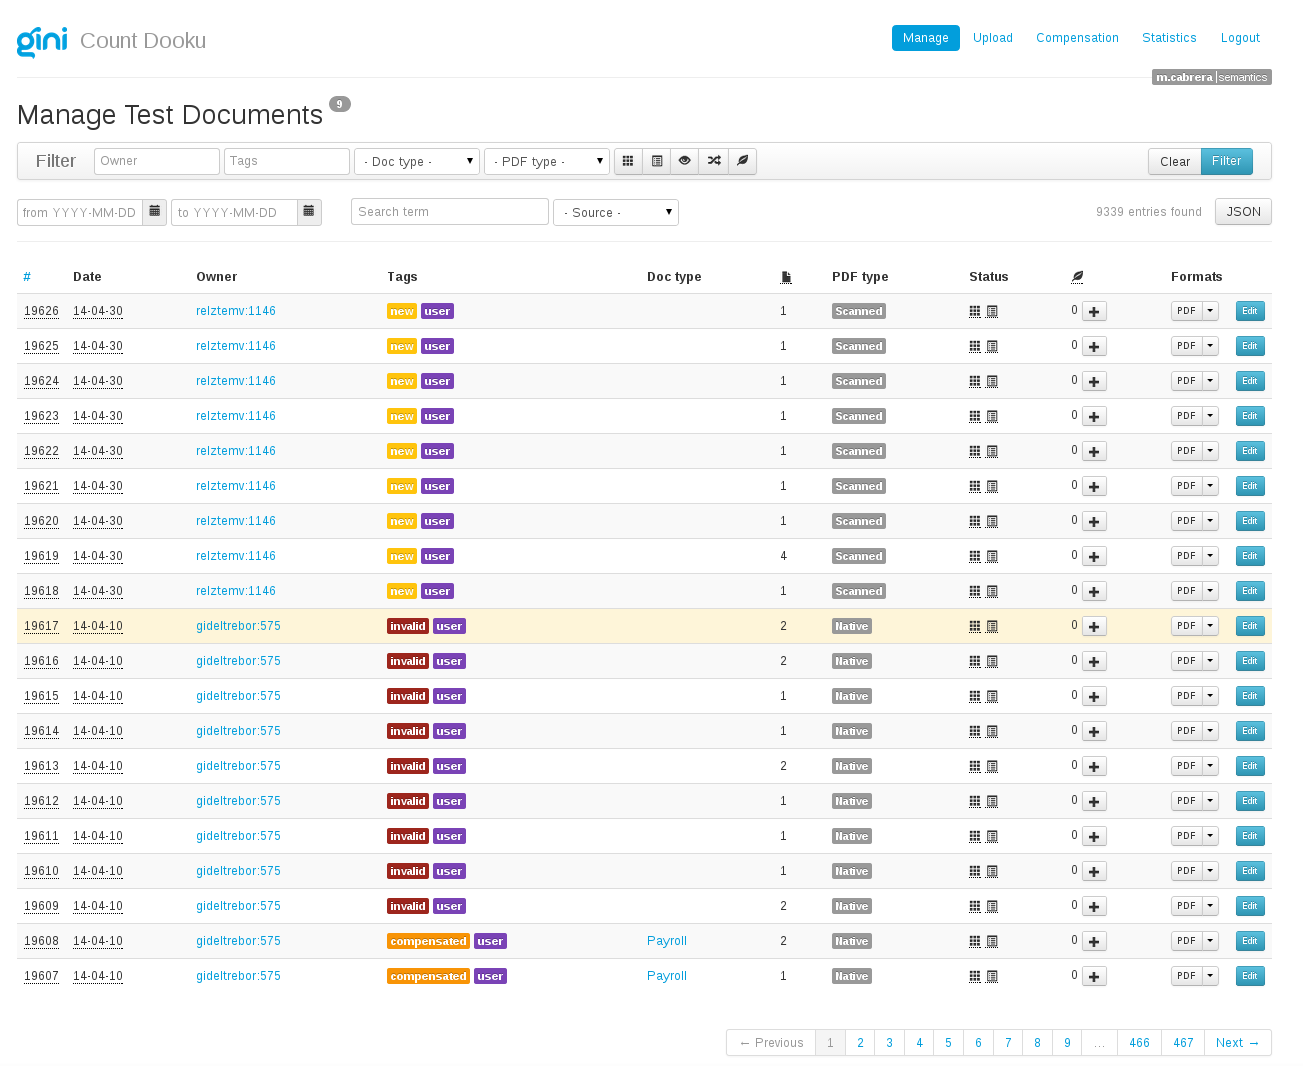
\includegraphics[width=\textwidth]{images/001-dooku-screenshot.png}
    \caption{Dooku - Gini document storage platform.}
    \label{fig:dooku_screenshot}
\end{figure}

\section{Gini document platform}
\label{sec:gini_doc_platform}

Gini currently owns a database  German language document. These documents 
are personal and business related documents that have been bought 
from  persons all over Germany. Document types are very broad and go from
long insurance contracts to short remittance slips. These document are stored
in a central system database that can be accessed via an  \texttt{API}.
Document can be either \textit{native} or \textit{scanned}. The document
\textit{native} that are native are orignal digital document. (e.g. PDF document) that
are uploaded to the system. \textit{Scanned} documents on the other hand, are
uploaded from an image obtained a scanner or a camera (e.g. a mobile phone
camera). Given the variability of the capture devices for the scanned
documents, the quality of such images is not regular among all the documents.
This is important to consider, given that after being uploaded all the
documents are processed using a \ac{OCR} solution, so the quality of the
images affect the the accuracy with which the text is extracted from. 
After the text has been extracted, it is stored  along with
the position of the words on the page; font size and style,  and other information a into a database using a custom
\textsc{XML} format.  Besides this information, a document is also assigned
\textit{tags} or labels, that when querying for particular characteristic
(e.g. quality, source, etc.) help filter the results. Figure
\ref{fig:dooku_screenshot} shows a screen-shot of the application with the
most important columns.


After being stored and preprocessed, this document are annotated by a human.
The annotations include labels such as  \textit{sender name}, \textit{bank
  account} (in the case of financial documents), \textit{amount to pay} and
\textit{document type} (\ac{DocType}). Using this annotation several
machine leaning algorithm are trained.  These classifier are then exposed to
clients also via an \texttt{API}. Table \ref{tab:list_gini_doctypes} shows the
complete list of \ac{DocTypes} available in the system and their description.


\section{The Gini Document Classifier}  
\label{sec:gini_doctype_classifier}

One of the functionality that Gini offer to their customer is document
classification.  As mentioned in the previous section this is done using
machine learning on top of the annotations made by humans. In the particular
case of the \ac{DocType} classifier, it is implemented using \ac{SVM} using
handcrafted features such as the appearance of a particular word, the font
of specific words, the number of pages of the documents, etc. This features
once constructed are fed into the \ac{SVM} implementation to train classifier. the
classifier is then exposed through a Web service.

The particular implementation of the \ac{SVM} is based on \texttt{Java}
implementation of the popular \texttt{LIBSVM} \cite{CC01a} using a
\texttt{RBF} Kernel.  The training is done using grid search and the best
model in 10-fold cross-validation with all the training data available is
taken.

There are some external an internal challenges that this classifier is faced
with:

\begin{itemize}
\item The quality of the data: As much of the data comes from varying degree
  of capture devices, the quality of the OCR is not perfect, thus producing a
  lot of noise in the stored text.
\item Feature generation and extension: Every time a new document type is
  required to be supported, a manual analysis of the document type should be
  done with the purpose of identifying what features are important and then
  these are added to the document.
\item No validation of the classifier is done on a validation set and quality
  is measured on documents belonging to the training set. This fundamental
  flaw, albeit obvious in a scientific setting, is many times overlooked in
  the industry.
\end{itemize}

Taking in consideration all these challenges, the objective is then to design
a better classifier that allow, at least partially, solve the
aforementioned issued.



\section{Experiments}
\label{sec:w2vec_doctype_experimental_setup}

As mentioned in the introduction, three different approaches are going to be
compared, namely:

\begin{itemize}
\item The current \ac{SVM} implementation with the handcrafted features.
\item A new \ac{SVM} implementation using \ac{BOW} features.
\item A new \ac{SVM} implementation using \textit{Word2vec} word vector as features.
\end{itemize}

The classification algorithm is kept while the
evaluation real evaluation is on the features. The idea  is to verify
that in fact better features account for better classification. The following
sections describe each of the features and the specific od the algorithm. 


\subsection{Gini Document Database and Dataset Description}
\label{sec:gini_db_dataset_desc}
  
Section \ref{sec:gini_doc_platform} described briefly the platform where
document Gini owned resided. This section described the specific of the
documents used for training the classifier. 

Gini database of documents consists of approximately 9339 different types of
document, from these only 2685 are used to train the document classifier.
Table \ref{tab:doctype_classifier_classes} show the distribution of the data
set among the classes. As can be seen from the data set, not all classes
used. Furthermore, there is a class called \textit{Other} that include
documents that do not fall into any of the categories listed. It is also a
unbalanced data set, having with number of intances per class ranging from 69
to 650. All the document are not used in the data set because as of right now
it is not necessary to classify all of other classes (creating thus a large
unbalanced \textit{Other} class). Additionally, other document are not
annotated or annotated wrongly, that is, they are correct document but has
not been properly annotated with the correspondent \ac{DocType}.


\begin{table}[h]

  \centering
  \caption{Distribution of document type in  Gini \ac{DocType} classifier training set.}
  \label{tab:doctype_classifier_classes}

\small
\begin{tabular}{|l|c|}
\hline
 \textbf{Document Type}    &  \textbf{\# Instances}  \\
\hline
 CreditCardStatement  &           158  \\
 Other                &           650  \\
 BankStatement        &           369  \\
 Contract             &           178  \\
 InsurancePolicy      &           105  \\
 Payroll              &            69  \\
 Invoice              &           570  \\
 Reminder             &           596  \\
\hline
 Total                &          2685  \\
\hline
\end{tabular}
\end{table}

As mentioned mentioned previously, there was not an official test set used to
evaluate the classifier performance. Therefore a new one was defined using a
stratified random selection of 20\% original  set for the testing and the
other 80\% for training, ending up with 2156 documents for training  539 for
testing. The same documents are used to evaluate all the classifier /
features.


\subsection{Handcrafted Features}
\label{sec:sub_w2v4tc_current_features}

As mentioned back in section  \ref{sec:gini_doctype_classifier} the current
Gini document classifier is based  \texttt{LIBSVM} \cite{CC01a} using 
\texttt{RBF} Kernel.   The features used to rain this classifier are
handcrafted features that count then number of words (actually the matches of
specific regular expressions) in the text, the font size of some
words, the digit character ration, the average font size, etc. In total 701 features like these are used.
 

\subsection{\ac{BOW} Features}
\label{sec:sub_w2v4tc_bow_features}

For the \ac{BOW} features, the traditional \ac{tf-idf}  
\cite{Salton88term-weightingapproaches}\cite{Sebastiani02} discussed in
section [LINK TO RELATED WORK] is used as features. For the actual feature
extraction the \texttt{TfidfTransformer} from \texttt{Scikit-learn}
\cite{scikit-learn}  was used ending up with 55122-dimensional sparse
vectors.

As for  pre-processing for feature extraction,  typical stop word subsitution was performed with the help
of \ac{NLTK} \cite{BirdKleinLoper09}. Additional stop word clean up was
detected by looking at the vocabulary, for example extremely large words
(more than 30 characters) and word containing non German alphanumerical
characters were verified that were not the result of wrong OCR
readings and were removed accordingly. In addition to this, words than
appeared in 90\% of the documents were removed  previous the \ac{tf-idf}
feature generation.


As for  pre-processing for feature extraction,  typical stop word subsitution was performed with the help
of \ac{NLTK} \cite{BirdKleinLoper09}. Additional stop word clean up was
detected by looking at the vocabulary, for example extremely large words
(more than 30 characters) and word containing non German alphanumerical
characters were verified that were not the result of wrong OCR
readings and were removed accordingly. In addition to this, words than
appeared in 90\% of the documents were removed  previous the \ac{tf-idf}
feature generation.



\subsection{Word Vector  based Features}
\label{sec:sub_w2v4tc_w2v_based_features}

As mentioned early in the document, using word vector features form \ac{TC}
posses some challenges from the algorithm point of view. Although in theory
we could represent a document as the concatenation of all the vector
representation of the words in contains, this in practice would be impossible
as first each document has a different number of words which would imply
high-dimensional variable size dense vector representing a document that
could not be used to train with traditional learning algorithm and in
particular the current classification algorithm used by Gini.

Another approach described in previous work named \textit{document mean
  representation} consists of average of the vector representation of the  words
present in the document.  More formally, assuming that there is  vocabulary of
size $|V|$ and with learned $\beta$-dimensional word vector representation of
that vocabulary, then  $R  \in \mathbf{R}^{(\beta \times |V|)}$  is  the
matrix of learned word vectors.  The representation of a document $d \in |V|$ can be obtained using the following method:

$$d = Rv$$

Where $v$ is a $|V|$-dimensional  binary vector representation of the
document.   The resulting vector $d$ is then  normalized or the mean can be
applied (hence the name mean).

%Also the word representation matrix $R$ is also   normalzed using the work of [1]  

Although simple in principle, these document representation has  shown good
results task such as sentiment analysis and even an improvement when used in tandem
with more traditional document representation  \cite{maas2010probabilistic},
event though In the cited referenced, they used another word vector representation that
did not have the linear compositionality characteristic of the
\textit{Word2vec} generated word representation \cite{MikolovSCCD13}.


\subsubsection{Training of the Word Vector Features}
\label{sec:sub_w2v_4tc_training-word-vector}
In order to use word vector representations to do document classification it is necessary to train the
vectors.  As all the documents of the document classification training set are
in German a German language word vectors are needed.  One option a
corpus like the German Wikipedia is necessary. However, as mentioned back in
chapter \ref{chapter:wor2vec_german} the nature of the text the word vectors
are generated from influences the quality of the word vectors and their
performance in specific tasks. For that reason, the whole unlabeled document
database that  Gini are used to generate the word vector used for document
classification. 

The data from Gini document is stored as \texttt{XML} documents in a
relational database. These document were exported and preprocessed. Besides
the text, the format contains the coordinates of the position of each word
existing in the document. This information is not necessary for the purpose
and is therefore removed. In addition, the preprocessing described back in
section \ref{sec:adapt_task_german_lang} is also applied to this dataset.

Table \ref{tab:w2v4tc_dataset_comparisson} compares the two data sets used
to generate the document classification. There is a big difference in
vocabulary and number of token trained. However, as it will be in the result
section this does not necessarily mean that for this particular tasks the
word vector generated from Wikipedia will be necessarily superior.

\begin{table}[h]

  \centering
  \caption{Comparisson of the datasets used to train the word vector for
    \ac{DocType} classification}
  \label{tab:w2v4tc_dataset_comparisson}

\small
\begin{tabular}{|l|c|c|c|}
\hline
Dataset           &  Size (MB)  &    \# Tokens  &  Vocabulary  Size  \\
\hline
 Gini Dataset      &         27  &     3657159  &             33596  \\
 Wikipedia German  &       6656  &  1051584822  &           1871739  \\
\hline
\end{tabular}

\end{table}


\section{Training and Evaluation}

For the handcrafted features and \ac{BOW} based classifier a standard 10-fold
cross-validation  on the training data  was used to select the best model.
As mentioned in section \ref{sec:gini_doctype_classifier}, this classifier is
based on  on \texttt{LIBSVM} \cite{CC01a}.
Afterwards the classifier were evaluated on the testing set and based on
those results are compared against each other.

For the \ac{BOW} feature based classifier as well as for the word vector
based one, the  \texttt{SVC} implementation of  \texttt{Scikit-learn}
with a linear kernel and automatic class weights was used. This
implementation is also  based on \texttt{LIBSVM}. However, after evaluating
other implementation, the  faster \texttt{LinearSVC} based on \texttt{LIBLINEAR}
\cite{Fan:2008:LLL:1390681.1442794}  produced better faster training times
and slightly better results. This classifier was also tested on the
handcrafted features but there was a significant loss in performance.


For the \textit{document mean representation} we had two possible dataset to
train the word vector from from. For the Wikipedia corpus we selected the model that
performed the best as describe in section \ref{experiments:sub:evaluation}. 
As for the word vector generated from Gini dataset 
size of the dataset  allowed a fast model generation. So around 120
\textit{Word2vec} model generation  combinations. All these combinations
were trained using the same 10-fold cross-validation to set the parameters on
the classifiers and then evaluated on testing set.


The evaluation measures are the standard measures used in document
classification: \textit{precision}, \textit{recall}, \textit{f-score}. These
measures are  weighted to account for unbalanced in the classes. These
performance measures are described in detail back in section [LINK TO SECTION].


\begin{table}[h]

  \centering
  \caption{Top-5 of evaluation of document classification task using
    \textit{document mean representation} generated from word vectors learned
  using Gini unlabeled dataset. The model were trained using a subsampling of
  $10^{-5}$.}
  \label{tab:w2v4tc_ginig_w2v_evaluation}

\small
\begin{tabular}{|c|c|c|c|c|c|c|}
\hline
 Algorithm  &  Architecture  &  Window  &  Dim.  &  Precision  &    Recall  &  F1-Score  \\
\hline
 \ac{HS}    &  Skip-gram     &      15  &   340  &   0.916914  &  0.914657  &  0.914861  \\
 \ac{HS}    &  Skip-gram     &      15  &   160  &   0.914635  &  0.912801  &  0.912901  \\
 \ac{HS}    &  Skip-gram     &      15  &   200  &   0.912762  &  0.910946  &  0.911149  \\
 \ac{HS}    &  Skip-gram     &      10  &   460  &   0.910683  &  0.909091  &  0.909243  \\
 \ac{HS}    &  Skip-gram     &      15  &    80  &   0.909976  &  0.909091  &  0.909231  \\
 \ac{HS}    &  Skip-gram     &      15  &   240  &   0.909967  &  0.909091  & 0.909075  \\
\hline
\end{tabular}
\end{table}


Table \ref{tab:w2v4tc_ginig_w2v_evaluation} shows the TOP-5 model for Gini  data set evaluated on the
testing set. 


\section{Results}
\label{sec:w2v4tc_results}

This section compares the different 



% Table comparing the best result of each approach.
% The cross validation results.
% the t-SEN plots of the features.
% training with wikipedia and comparisson
% The graph of generalization vs less trained data.
 

\begin{figure}[h]
    \centering
    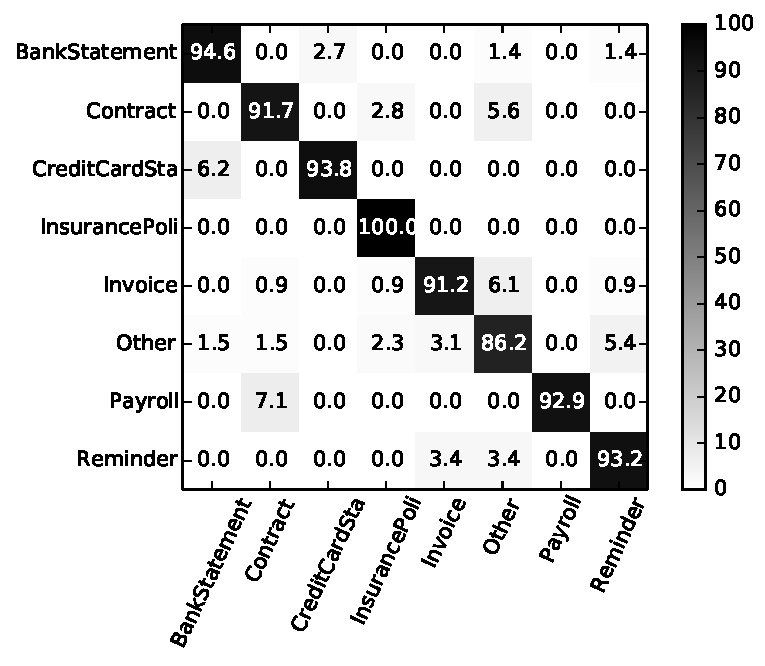
\includegraphics[width=0.7\textwidth]{images/002-xvalidaton-dmr.pdf}
    \caption{Confusion matrix of the classification results  using \textit{document mean
      representations} features - Values of percentages of the test set per
    each document type.}
    \label{fig:confusion-matrix-dmr}
\end{figure}


\begin{figure}[h]
    \centering
    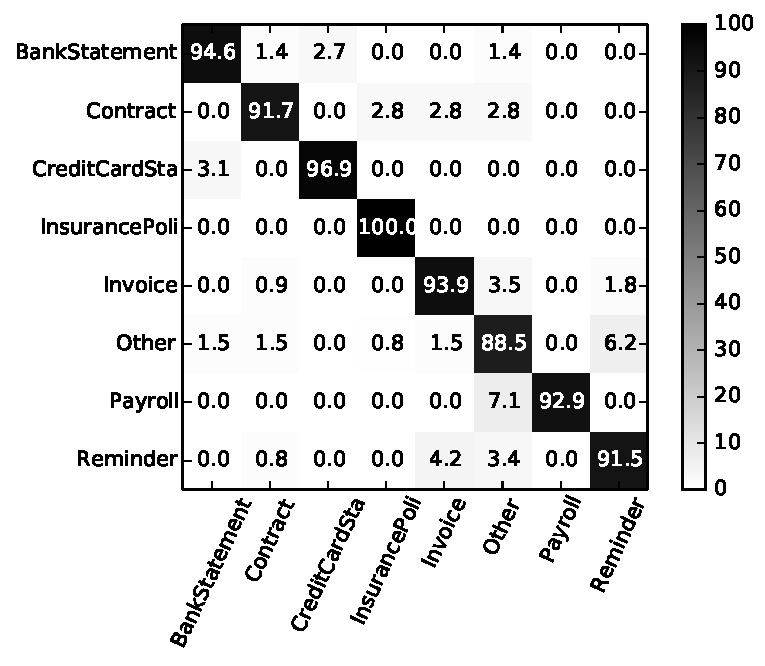
\includegraphics[width=0.7\textwidth]{images/003-xvalidaton-bow.pdf}
    \caption{Confusion matrix of the classification results  using \textit{document mean
      representations} features - Values of percentages of the test set per
    each document type.}
    \label{fig:confusion-matrix-bow}
\end{figure}




\begin{figure}[h]
    \centering
    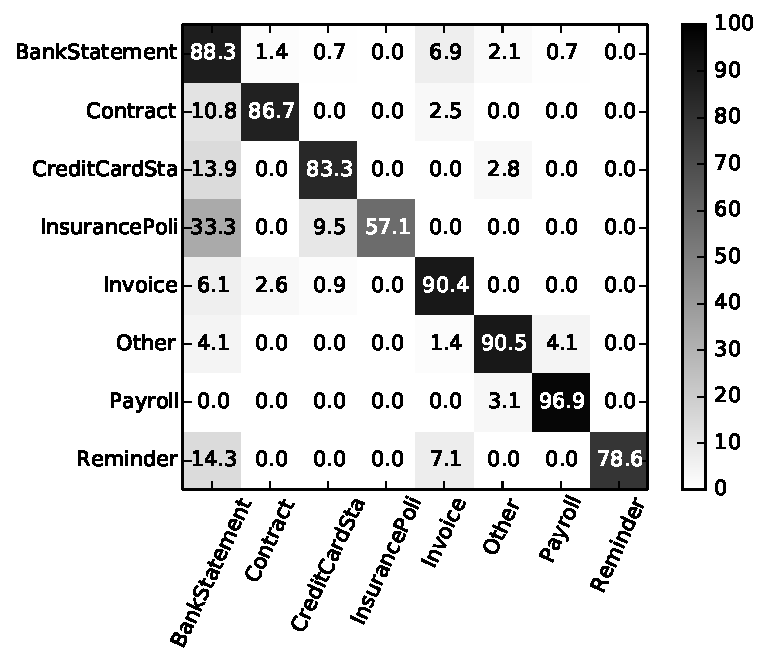
\includegraphics[width=0.7\textwidth]{images/004-xvalidaton-handcrafted.pdf}
    \caption{Confusion matrix of the classification results  using \textit{document mean
      representations} features - Values of percentages of the test set per
    each document type.}
    \label{fig:confusion-matrix-handcrafted}
\end{figure}





\section{Conclusion}
\label{sec:w2v4tc_conclusion}
blah 


%Once the word vector are generated 
 

% The training is done using grid search and the best
% model in 10-fold cross-validation with all the training data available is%
% taken.



%Discussion - Promise of Deep Learning and modifiy the word vectors.



% - Stored Dookud
% - Stored as DocXML not only text but also location information of words.
% - Two ways to get the text from the document {Native, Scanned (e.g.)}

%  approach as well as the most
% important results. It includes  a performance comparison of the word vectors in German with their counterpart in English as well as  the evaluation of  some corpus
% preprocessing approaches that might affect the performance of the word
% representation for German.


      %\caption{List of document types available in Gini Dataset}
      %\label{tab:list_gini_doctypes}
%\begin{tabular}{|c|p{8cm}|}


% \begin{longtable}[h]{|l|p{9cm}|}
% \caption[List of document types available in the Gini Dataset]{List of document types available in the Gini Dataset} \label{tab:list_gini_doctypes} \\
% \hline DocType code & Description \\
% \hline Administrative\_offence                  &  Administrative offence - Administrative Rechnungen, wie z.B. Strafzettel, Bu{\ss}geldbescheide      \\
%  admission\_ticket                        &  Admission ticket -  Eintrittskarte                                                                \\
%  airline\_ticket                          &  Airline ticket -  Flugticket (Boardkarte, Buchung)                                                \\
%  bank\_statement                          &  Bank statement -  Kontoauszug                                                                     \\
%  confirmation\_of\_termination            &  Confirmation of termination -  K\"{u}ndigungsbest\"{a}tigung                                  \\
%  contract                                 &  Contract -  Vertrag                                                                               \\
%  contract\_confirmation                   &  Contract  confirmation -  Best\"{a}tigung Vertrag (alle Dom\"{a}nen)                          \\
%  contract\_energy                         &  Contract  energy  - Energie (Vertrag)                                                             \\
%  contract\_extension                      &  Contract  extension -  Vertragsverl\"{a}ngerung                                                 \\
%  contract\_insurance\_automobile          &  Contract insurance automobile -  Kfz-Versicherung (Vertrag)                                       \\
%  contract\_insurance\_household           &  Contract insurance household -  Hausratversicherung (Vertrag)                                     \\
%  contract\_insurance\_legal\_costs        &  Contract insurance legal costs - Rechtsschutz (Vertrag)                                           \\
%  contract\_insurance\_third\_party\_risk  &  Contract insurance third party risk  - Haftpflicht (Vertrag)                                      \\
%  contract\_telco                          &  Contract telco -  Telko (Vertrag)                                                                 \\
%  credit\_card\_statement                  &  Credit card statement - Kreditkartenabrechnung                                                    \\
%  credit\_note                             &  Credit note -  Gutschrift
%  \\ 
%  delivery\_note                           &  Delivery note -  Lieferschein                                                                     \\
%  insurance\_policy                        &  Insurance policy -  Versicherungsunterlagen                                                       \\
%  invoice                                  &  Invoice - Rechnung                                                                                \\
%  lease\_contract                          &  Lease contract -  Mietvertrag Leasingvertrag                                                      \\
%  letter                                   &  Letter  Brief - (interessante Doks f\"{u}r die es keinen DocType gibt)                          \\
%  medical\_finding                         &  Medical finding - Medizinischer Befund                                                            \\
%  medical\_insurance                       &  Medical insurance -  Krankenversicherungsdokument                                                 \\
%  notice\_of\_termination                  &  Notice of termination -  K\"{u}ndigung                                                          \\
%  offer                                    &  Offer -  Angebot                                                                                  \\
%  order\_confirmation                      &  Order confirmation  - Bestellbest\"{a}tigung, Auftragsbest\"{a}tigung                         \\
%  payroll                                  &  Payroll -  Gehaltsabrechnung                                                                      \\
%  receipt                                  &  Receipt  - Kassenzettel                                                                           \\
%  reminder                                 &  Reminder  Mahnung                                                                                 \\
%  remittance\_slip                         &  Remittance slip -  \"{U}berweisungstr\"{a}ger                                                 \\
%  return\_form                             &  Return form -  R\"{u}ckgabeformblatt (z.B. ecommerce amazon)                                    \\
%  social\_security\_statement              &  Social security statement -  Sozialversicherung, Meldebescheinigung zur Sozialversicherung        \\
%  statement\_energy\_consumption           &  Statement energy consumption -  Verbrauchsabrechnung (Strom, Gas, Wasser, etc)                    \\
%  statement\_pension                       &  Statement pension -  Rentenbescheid, Rentenversicherungsunterlagen                                \\
%  stock\_document                          &  Stock document -  Wertpapierdepotausz\"{u}ge, Dividendenabrechnungen, Orderbest\"{a}tigungen  \\
%  tax\_assessment                          &  Tax assessment  Steuerbescheid                                                                    \\
%  tax\_document                            &  Tax document -  Lohnsteuerbescheinigung, Best\"{a}tigung f\"{u}r die Steuererkl\"{a}rung    \\
%  tax\_return                              &  Tax return -  Steuererkl\"{a}rung                                                               \\
%  taxi\_receipt                            &  Taxi receipt - Taxi-Quittung                                                                      \\
%  terms\_and\_conditions                   &  Terms and conditions -  Gesch\"{a}ftsbedingungen                                                \\
%  travel\_expense\_report                  &  Travel expense report - Reisekostenabrechnung     \\             \hline                          
% \end{longtable}



%%% Local Variables: 
%%% mode: latex
%%% TeX-master: "../main.tex"
%%% End:

                
\chapter{Conclusion and Future Work}
\label{chap:conclusion_future_work}

This master thesis studied the behavior of distributed representation learned by the \textit{Word2vec} model on German language data. It also evaluated and compared the learned distributed representations  against traditional handcrafted features for the classification of German language business document.
The evaluation of the word vector features included not only the analytically evaluation of the obtained word representations, but also the construction of a set  semantic and syntactic question in the German akin to the  one existing already for the English language. This is useful because it will allow other word vector model to evaluate the performance in the German language. The evaluation also yielded interesting results regarding the different factors affecting the performance of the \textit{Word2vec} model. For instance,  the impact of the semantic information contained in the corpus e learning the model. In particular, when building word representations that are topical smaller corpus of  text containing  with richer semantic relationships  are preferable to large amounts of text with no specific context. 
The study of the word vector representation showed that although the model
captured  semantic relationships correctly, for the syntactic tasks it was  not as successful. This can be explained by the morphological complexity of the German language in comparison to English. So, in order to capture properly these relationships it is necessary also to give the model more information about the morphological structure of the language.

In the context of document classification, the learned word vector
representations did   not outperform the state of the art  \ac{tf-idf}
features. However, they  did perform better than the handcrafted features on
the German language business document used for the evaluation. However, the
difference between  the performance measures is not large. This is relevant
if the amount of data used to train the model is taken into account. By
comparison,  the trained model by Google on the Google News dataset used
terabytes of Google news data. The model trained on Gini dataset contained
less than 100MB of information and yet they performed fairly similar. This
suggests that with more relevant data it is possible to learn better
representations, thus improving the performance of 
the document classifier. It is important to make emphasis on the word
\textit{relevant},  as a model trained on the German Wikipedia was also used
yielding good results as well but not outperforming either the  \ac{tf-idf}
features or the model learned on business documents.   However, this is a
good example of transfer learning were an unrelated dataset is used to learn
features that can be used to tackle a completely  different problem.


The features used to classify document were
just the averaged sum of word vector representation of the used documents.
Although it is reported that for long documents this will not yield good
results \cite{MikolovSCCD13},  for this particular problem they performed well 
well. Yet, more sophisticated word representation for long documents are needed in
order to account for the importance of words and the context.
 Recent work goes in this direction by obtaining 
fixed-length distributed representation of sentences and documents via an
unsupervised learning algorithm similar to \textit{Word2vec}, but in addition
having a paragraph matrix which represents the missing information from the
current context and act as memory of the topic of the paragraph
\cite{2014arXiv1405.4053L}. However, this only work so far for short
sentences / documents. Thus, techniques for obtaining distributed
representation of long documents are yet to be developed. 

Finally, given the nature of distributed representation, once the
unsupervised learning of the features is complete, further supervised fine-tuning can be
achieved using the specific tasks objective as evaluation function. This
particular problem has not been yet tackled for  word vector representations
in the context document classification, let alone for paragraph or long document representations.

% compared to the dataset used to learn the word vectors of 


% More results of the word vector
% Results from the document classification tasks
% Future of these techniques:
% Document representation
% ove the learned word vectors after  the unsupervised 
% chaining SVM 
 

% In this master thesis a framework for wifi data analysis was designed and implemented, providing tools for the localization of wifi APs, for continuous monitoring of statistical key parameters, and for the visualization of wifi related data. Different localization techniques where evaluated for their performance. The best performing algorithm, based on “Trilateration”, outperforms other state-of-the-art solutions with position es- timation accuracies between 6.75-47.10 meters and a median localization accuracy of 25.35 meters. The evaluation was based on a representative but limited dataset. The achieved state-of-the-art results may improve, given that the MeasrDroid data will em- body a bigger set of measurements, provided by a higher number of users. Also the position estimation errors are degraded by a high number of measurement errors in- duced by mobile phone hardware and real world abstractions. The position estimation can be further improved by embedding models better representing real world condi- tions and by collecting measurements from devices with better radio hardware.
% The statistical monitoring provides up-to-date and easily understandable representa- tions of important statistical key parameters, supporting the supervision of the systems state. The wifi visualization module provides sophisticated visual representation of the localized wifi APs in a geographic information system. Alltogether, the WAF provides a versatile toolset for the analysis of wifi related data.
% The work of this master thesis was only the first step towards continuously intercon- nected wifi networks. There is still a lot of work to be done. The evaluation conducted in this thesis was based only on a limited ground truth. For a thorough evaluation the ground truth has to be extended. Currently it comprises about 300 wifis, covering only 20% of localized wifi APs on average. Promising sources to extend the ground truth are the currently started home hot-spot program from Kabel Deutschland [33] or the upcoming home hot-spot program from the Deutsche Telekom [36].
% Further work has also to be done in the evaluation of localization techniques. This work only evaluated a small subset of possible techniques. Other approaches like prob- abilistic models or fingerprinting can possibly yield comparable or even better results.
% The WAF itself provides a huge set of possibilities for extensions. The wifi visual- ization module can be extended for example towars a wifi sensitive navigation system, which gives directions from a point A to a point B while providing the best wifi AP cov- erage along the way. Another possibility would be to extend the WAF to include GSM



%%% Local Variables: 
%%% mode: latex
%%% TeX-master: "../main.tex"
%%% End:

		
		% ---------------------------------------------------------------------------
		%
		% Appendix
		%
		% ---------------------------------------------------------------------------
		
		\part*{Appendix}
		\addcontentsline{toc}{part}{Appendix}
		
		\appendix %---------------------------------------
		
		\chapter{Detailed Descriptions}
%\section{Detailed Validation Results}
\label{chapter:DetailedDescriptions}
Here come the details that are not supposed to be in the regular text.
               

                \chapter*{Acronyms}
\begin{acronym}
    \acro{SVM}{Support Vector Machine}
    \acro{NNLM}{Neural Network Language Model}
    \acro{FNNLM}{Feedforward Neural Network Language Model}
    \acro{RNNLM}{Recurrent Neural Network Language Model}
    \acro{NLP}{Natural Language Processing}
    \acro{NN}{Neural Network}    
    \acro{TC}{Text Categorization}    
    \acro{IR}{Information Retrieval}  
    \acro{HS}{Hierarchical Softmax} 
    \acro{CBOW}{Continuos Bag of Words} 
    \acro{NLTK}{Natural Language Toolkit} 
    \acro{NER}{Named Entity Recognition} 
    \acro{VSM}{Vector Space Model} 
    \acro{OCR}{Optical Character Recognition} 
    \acro{DocType}{Document Type} 
    \acro{BOW}{Bag of Words}
    \acro{tf-idf}{term frequency-inverse document frequency} 
    \acro{t-SNE}{t-Distributed Stochastic Neighbor Embedding}
    \acro{CRF}{Conditional Random Fields}
 \end{acronym} 

                \addcontentsline{toc}{chapter}{Acronyms}


                
                 

\listoffigures
 
\listoftables
                 \addcontentsline{toc}{chapter}{List of Figures and Tables}
		
	


  \clearemptydoublepage
  
	\bibliography{bibliography/literature}
	
 
\end{document}


%%% Local Variables: 
%%% mode: latex
%%% TeX-master: t
%%% End: 
